\documentclass{beamer}

\usepackage[utf8]{inputenc}
\usepackage{csquotes}
\usepackage{latexsym,amsmath,xcolor,multicol,booktabs,calligra, animate, subfig}
\usepackage{graphicx,pstricks,listings,stackengine, bbm}
\usepackage{tikz}
\usetikzlibrary{fit,tikzmark}   
\usepackage{booktabs,cellspace}
\usepackage{color, colortbl}
\usepackage{hyperref}
\usepackage{color}
%Information to be included in the title page:
\title{Analysis of Utah's Proposed Regulation}
\author{Lauren Beatty\\ lbeatty@edf.org}
\institute{Environmental Defense Fund}
\date{September 21, 2023}
\logo{
\includegraphics[height=1cm]{EDF_color_printCMYK_2022.png}\hspace*{.03\paperwidth}\vspace{.01\paperwidth}}


%Color Pallete
\definecolor{EDFblue}{RGB}{0.0, 51, 204} % UBC Blue (primary)
\definecolor{EDFgreen}{RGB}{0, 153, 51} 
\definecolor{EDFlightgreen}{RGB}{161, 226, 20}
\definecolor{EDFcyan}{RGB}{51,204,255}
\setbeamercolor{structure}{fg=EDFblue} 
\setbeamercolor{button}{bg=EDFblue,fg=white}
\setbeamertemplate{navigation symbols}{}

% Override palette coloring with secondary
\setbeamercolor{subsection in head/foot}{bg=UBCgrey,fg=white}

\begin{document}

\frame{\titlepage}

\begin{frame}
\frametitle{Does the Proposed Regulation Sufficiently Cover Plugging Liabilities?}
    Compare hypothetical bond amounts by firm against:
    \begin{itemize}
        \item estimated plugging costs for \textit{all} wells
        \item estimated plugging costs for inactive/marginal wells.
    \end{itemize}
    Summary of findings:
    \begin{itemize}
        \item If plugging costs are high, then the proposed regulation doesn't cover total liabilities for many firms.
        \item \textit{However}, the proposed regulation does appear to sufficiently cover plugging liabilities for marginal/inactive wells for most firms.
        \item Meeting higher tier requirements can provide significant cost savings for operators.
    \end{itemize}
\end{frame}

\begin{frame}{Methods/Assumptions}
\label{BondCalc}
\vspace{-0.2cm}
To calculate firm-level bonds I conduct the following steps:
\begin{enumerate}
    \item For each well, sum production from 06/2022 until 06/2023 and classify each well as marginal ($<$2 BOE per day), active, or inactive.
    \item For each operator, calculate which tier they would fall in (determined by their percentage of inactive/marginal wells and total production for the year).
    \item Calculate the blanket bond and marginal/inactive depth well bond for each operator along with their per-well bonds for wells inactive $>12$ months.
    \item For operators that don't meet tier requirements (we call tier 4), calculate their total bonds as the sum of individual well bonds using the April draft of the proposed regulation.
\end{enumerate}
\hyperlink{bondingnumbers}{\beamerskipbutton{Individual Bond Numbers}}
\end{frame}

\begin{frame}{Methods/Assumptions}
\label{costcalc}
    To calculate estimate plugging costs I make four cost assumptions:
    \begin{enumerate}
        \item Assume each well costs $\$37,500$ to plug.
        \item Assume each well costs $\$75,000$ to plug.
        \item Assume each well costs $\$6$ per well-foot of depth to plug.
        \item Assume each well costs $\$12$ per well-foot of depth to plug.
    \end{enumerate}
    \vspace{.7cm}
    The estimates produced by assuming $\$6$ per foot look largely like the estimates produced from assuming $\$37,500$ per well.  Similarly, the estimates assuming $\$12$ per foot look largely like the estimates from assuming $\$75,000$ per well.

    \hyperlink{depths}{\beamerskipbutton{Well Depths}}
\end{frame}

\begin{frame}{If plugging costs are low, bonds cover total liabilities for many firms.}
\label{Fig1}
\begin{columns}
          \column{0.6\linewidth}
             \centering
             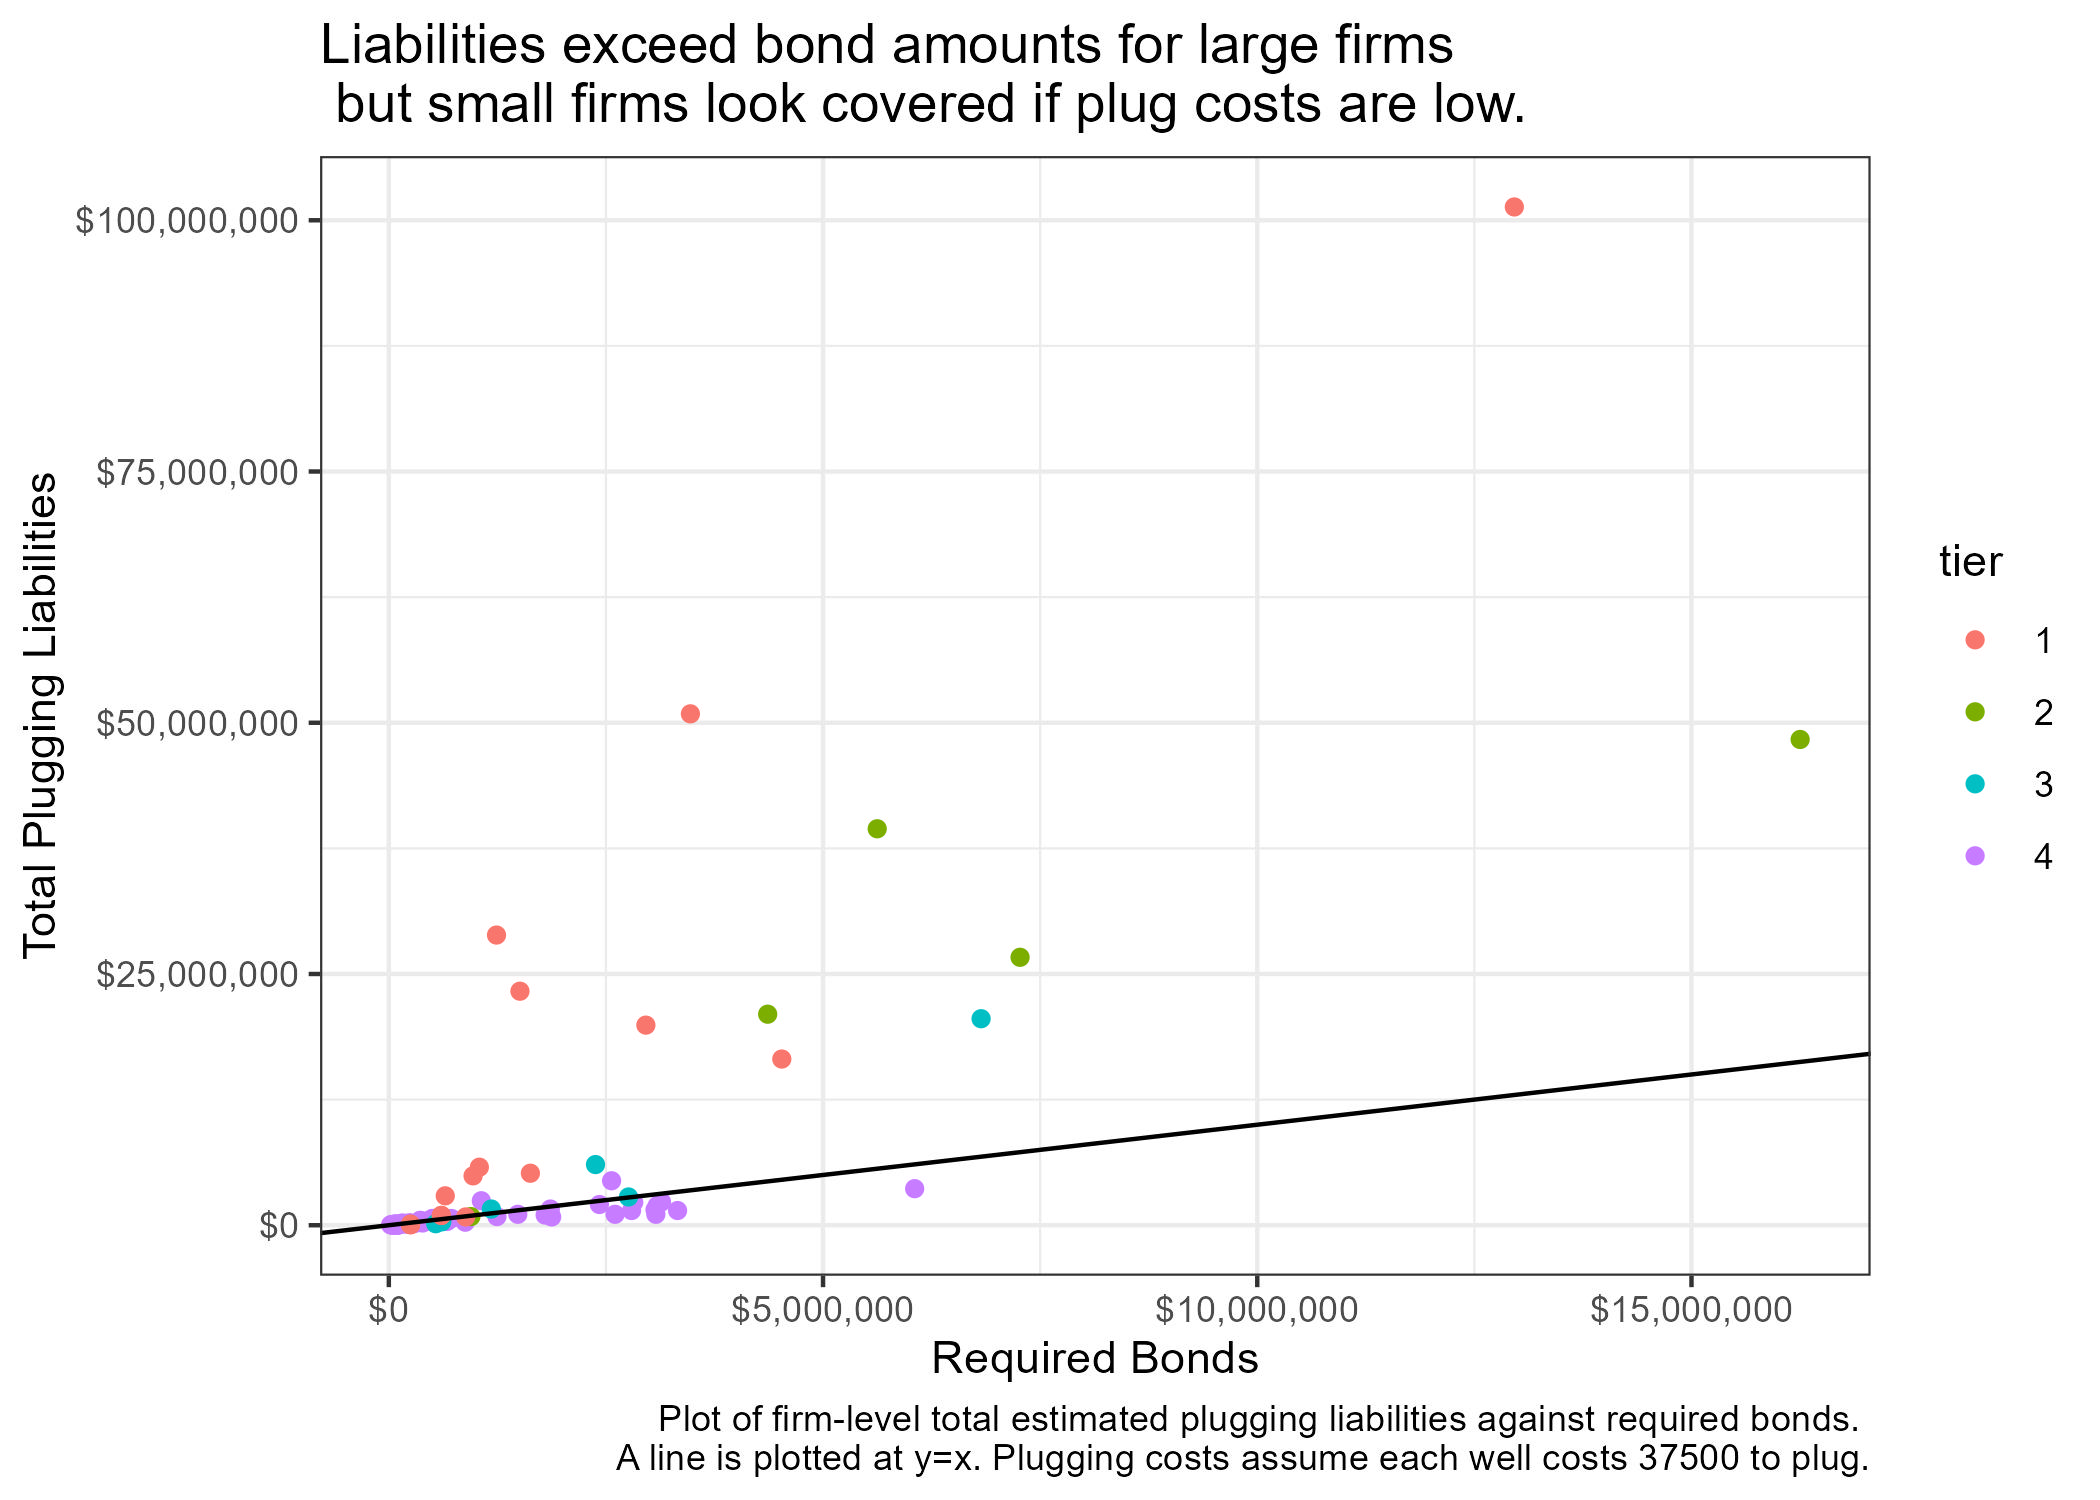
\includegraphics[width=1.08\textwidth]{Figures/BondsLiabilities1.jpg}
           \column{0.5\linewidth}
              \begin{itemize}
                  \item Dots above the line represent firms whose plugging liabilities exceed bonding amounts.
                  \item Firms that meet tier 1 and tier 2 requirements have significantly lower bond requirements than total plugging liabilities.
                  \item Smaller firms which don't meet tier requirements look well-bonded.
              \end{itemize}
\end{columns} 
\vspace{1cm}
\hyperlink{Liability1Zoom}{\beamerskipbutton{Zoomed}}
\end{frame}


\begin{frame}{If plugging costs are high, many firms have uncovered liabilities.}
\label{Fig2}
\vspace{-0.5cm}
\centering
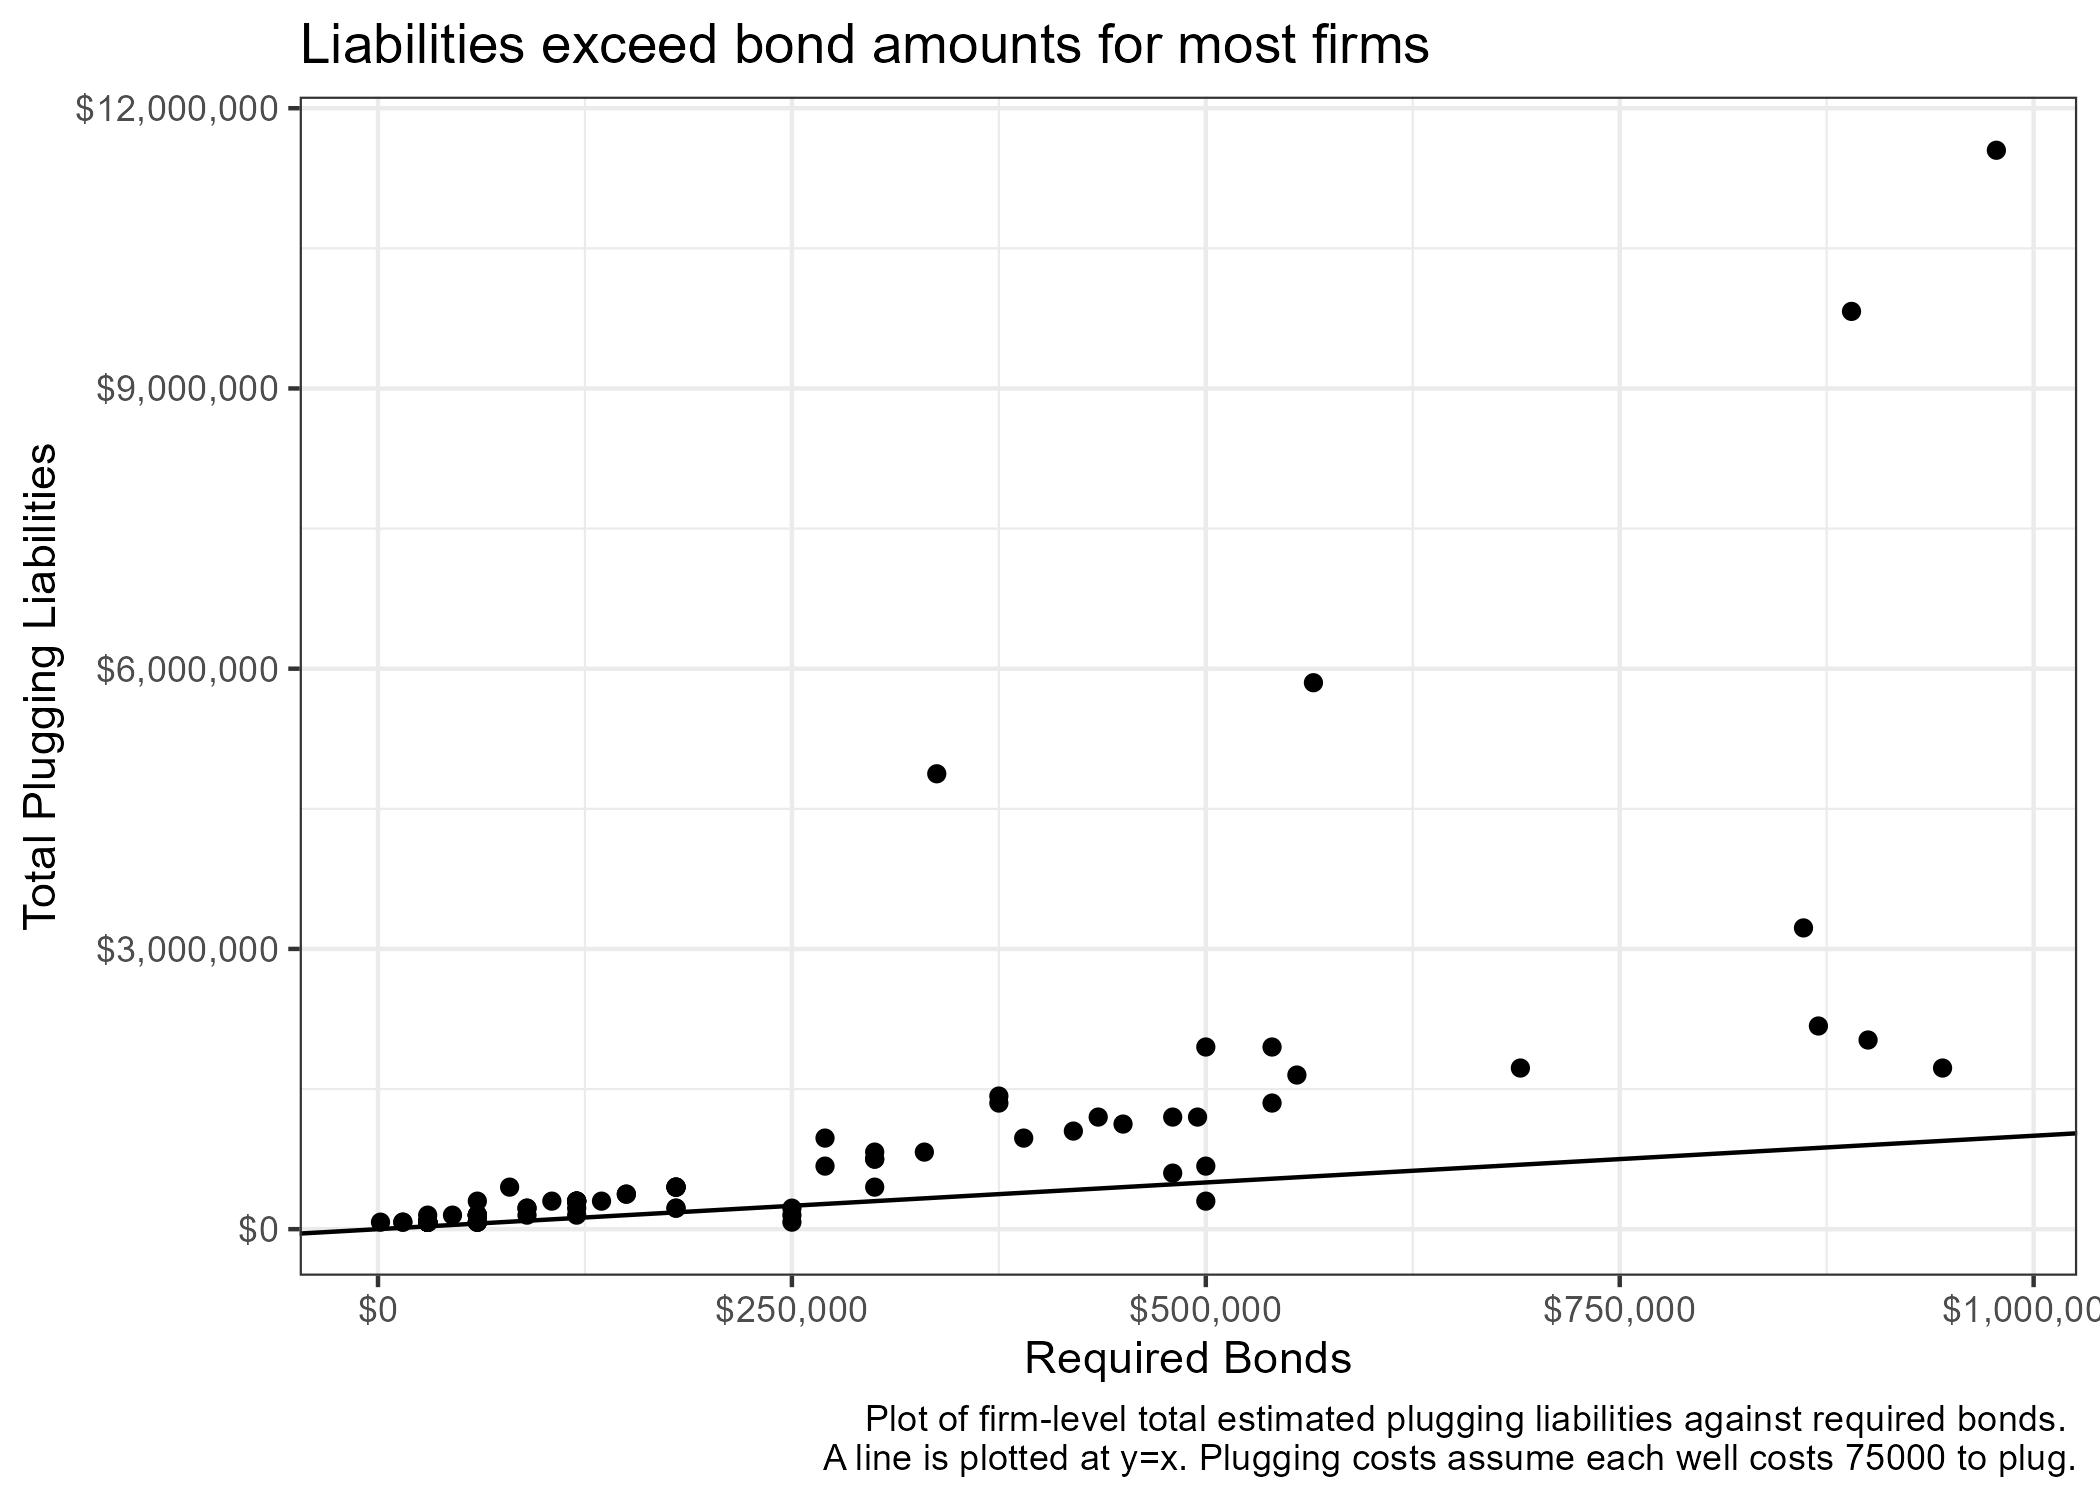
\includegraphics[width=0.8\textwidth]{Figures/BondsLiabilities2.jpg}

\hyperlink{Liability2Zoom}{\beamerskipbutton{Zoomed}}
    
\end{frame}

\begin{frame}{Even if plugging costs are high, the policy does a good job of covering liabilities from marginal/inactive wells.}
\label{Fig2Marginal}
\vspace{-0.5cm}
    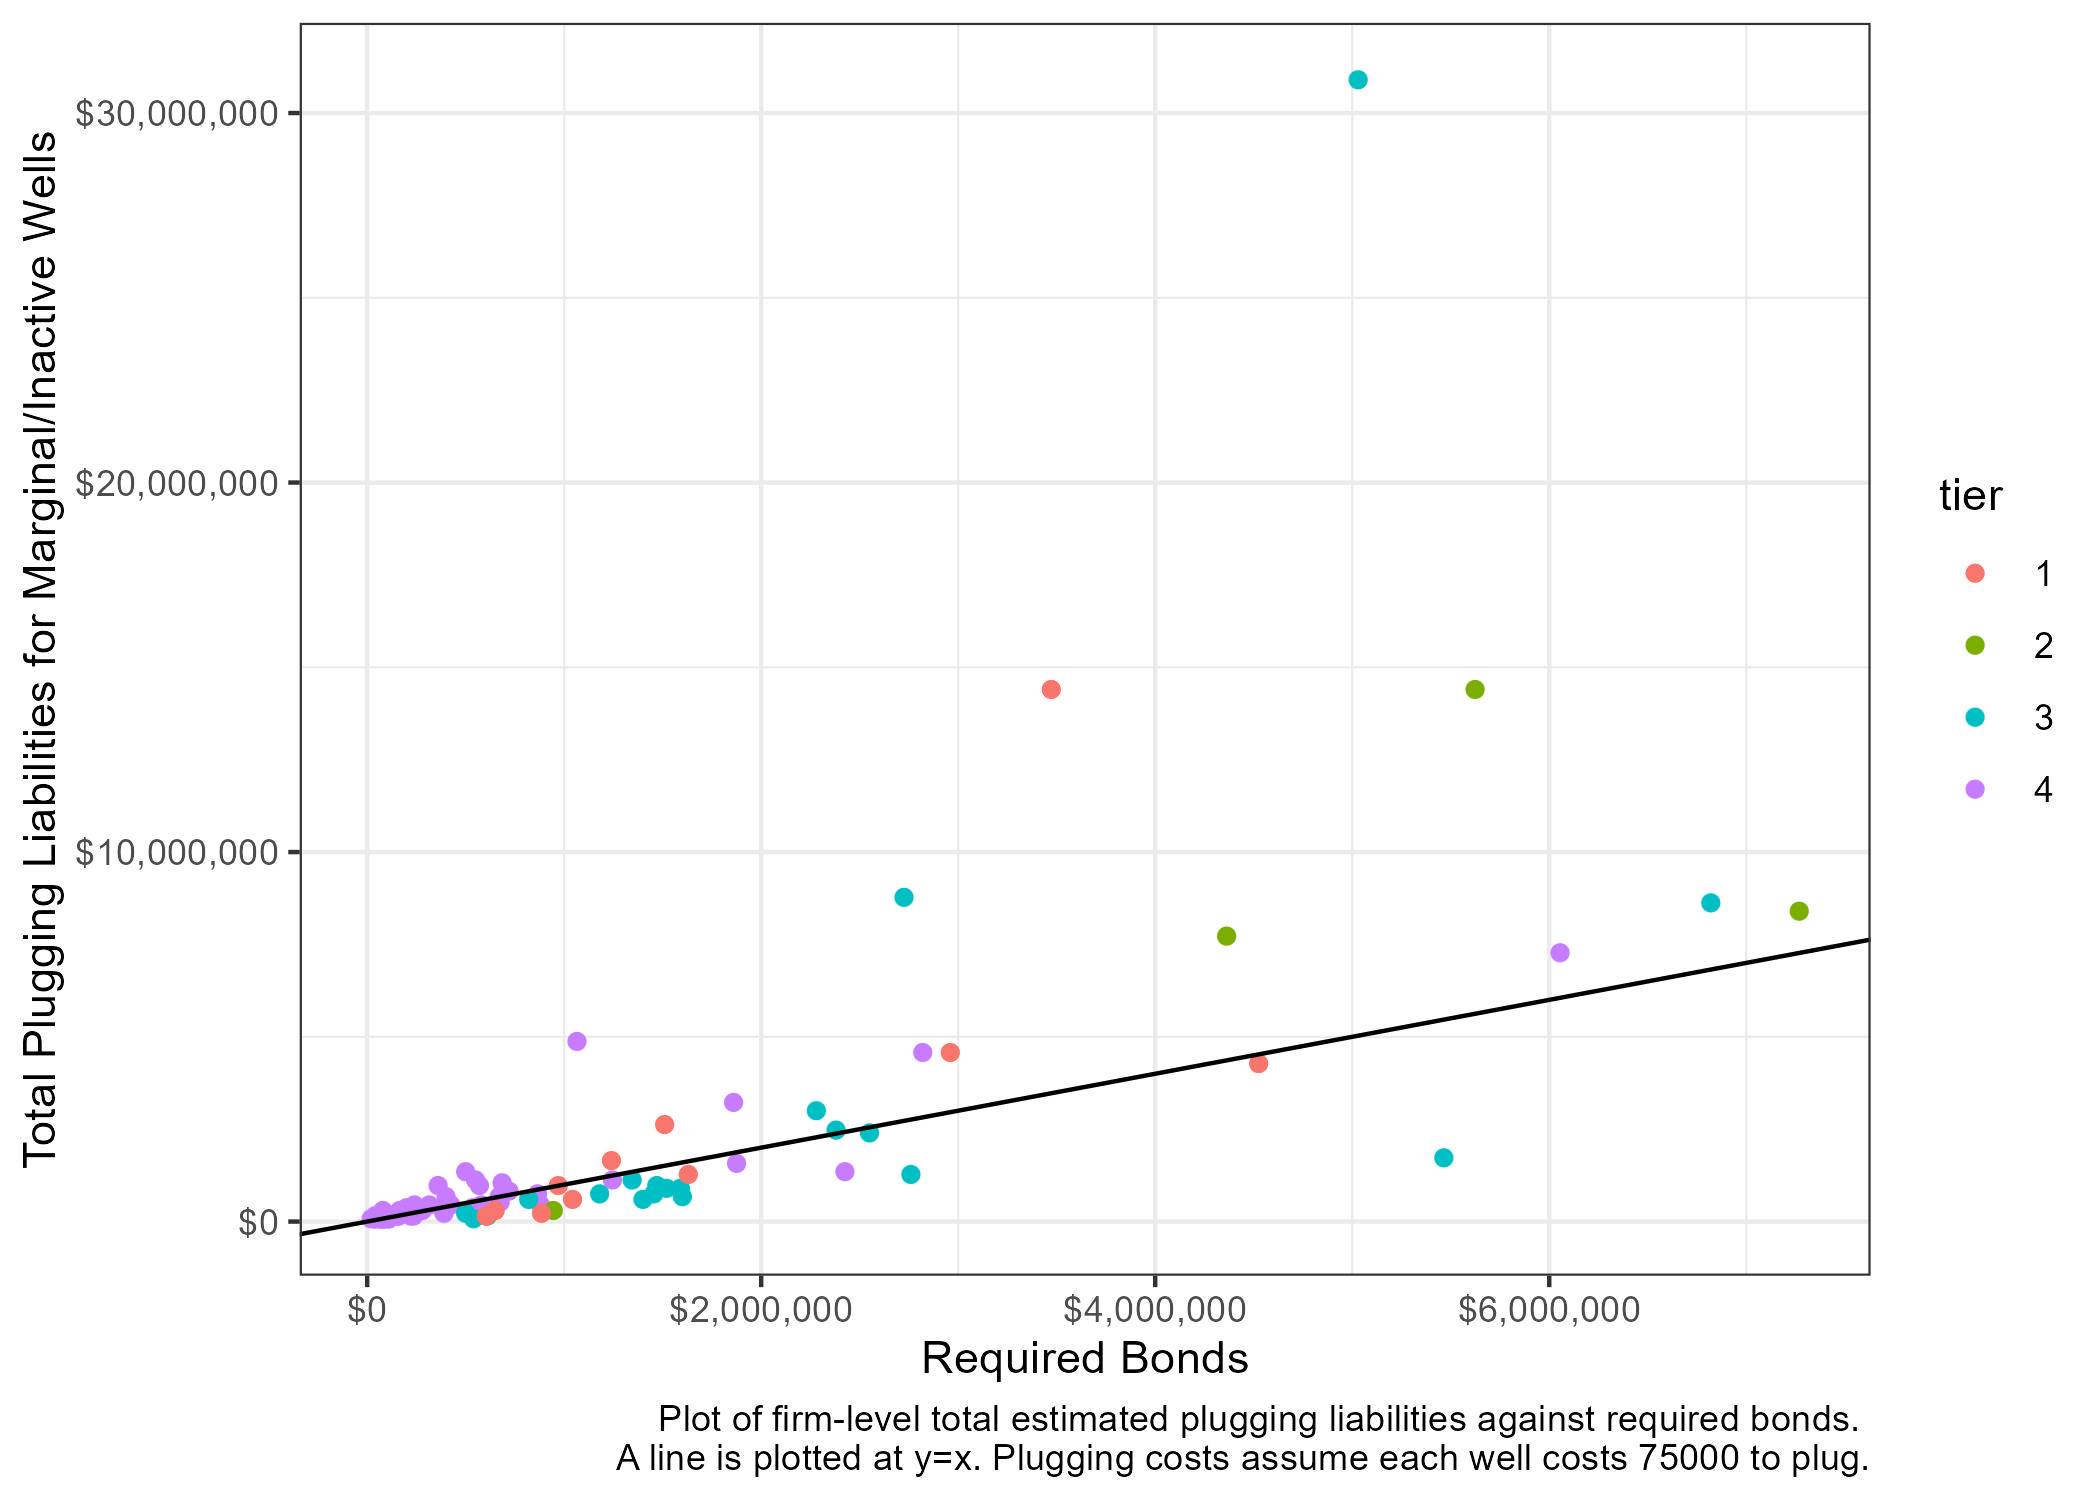
\includegraphics[width=0.8\textwidth]{Figures/InactiveMarginalLiabilities2.jpg}\\
    \hyperlink{Tier4Liability2}{\beamerskipbutton{Tier 4 Only}}

    
\end{frame}

\begin{frame}{Thanks!}
\label{Thanks}
    All of the code to reproduce these charts is available at: \href{https://github.com/lbeatty1/UtahDNRAnalytics}{https://github.com/lbeatty1/UtahDNRAnalytics}\\
    \vspace{1cm}

    Data is available from Utah DNR at:\href{https://oilgas.utah.gov/dataResearchCenter.php}{https://oilgas.utah.gov/dataResearchCenter.php}\\
    \vspace{1cm}

    Please feel free to contact me at:
    \href{lbeatty@edf.org}{lbeatty@edf.org}\\
    \vspace{1cm}

    Additional Content:
    \hyperlink{UPA}{\beamerskipbutton{UPA Tier Suggestions}} \hyperlink{MarginalInactiveLiability3}{\beamerskipbutton{Per-foot Cost Estimates}}
\end{frame}

\begin{frame}{Individual Well Bond Numbers}
\label{bondingnumbers}
\begin{table}[]
\begin{tabular}{l|l}
Depth                                      & Bond    \\
\hline
\leq 1,000                          & 10,000  \\
\textgreater{}1,000 and \leq 3,000  & 20,000  \\
\textgreater{}3,000 and \leq 6,000  & 40,000  \\
\textgreater{}6,000 and \leq 9,000  & 65,000  \\
\textgreater{}9,000 and \leq 12,000 & 85,000  \\
\textgreater{}12,000                       & 110,000
\end{tabular}
\end{table}
\hyperlink{BondCalc}{\beamerskipbutton{Back}}
    
\end{frame}

\begin{frame}{Well Depths}
\label{depths}
\centering
    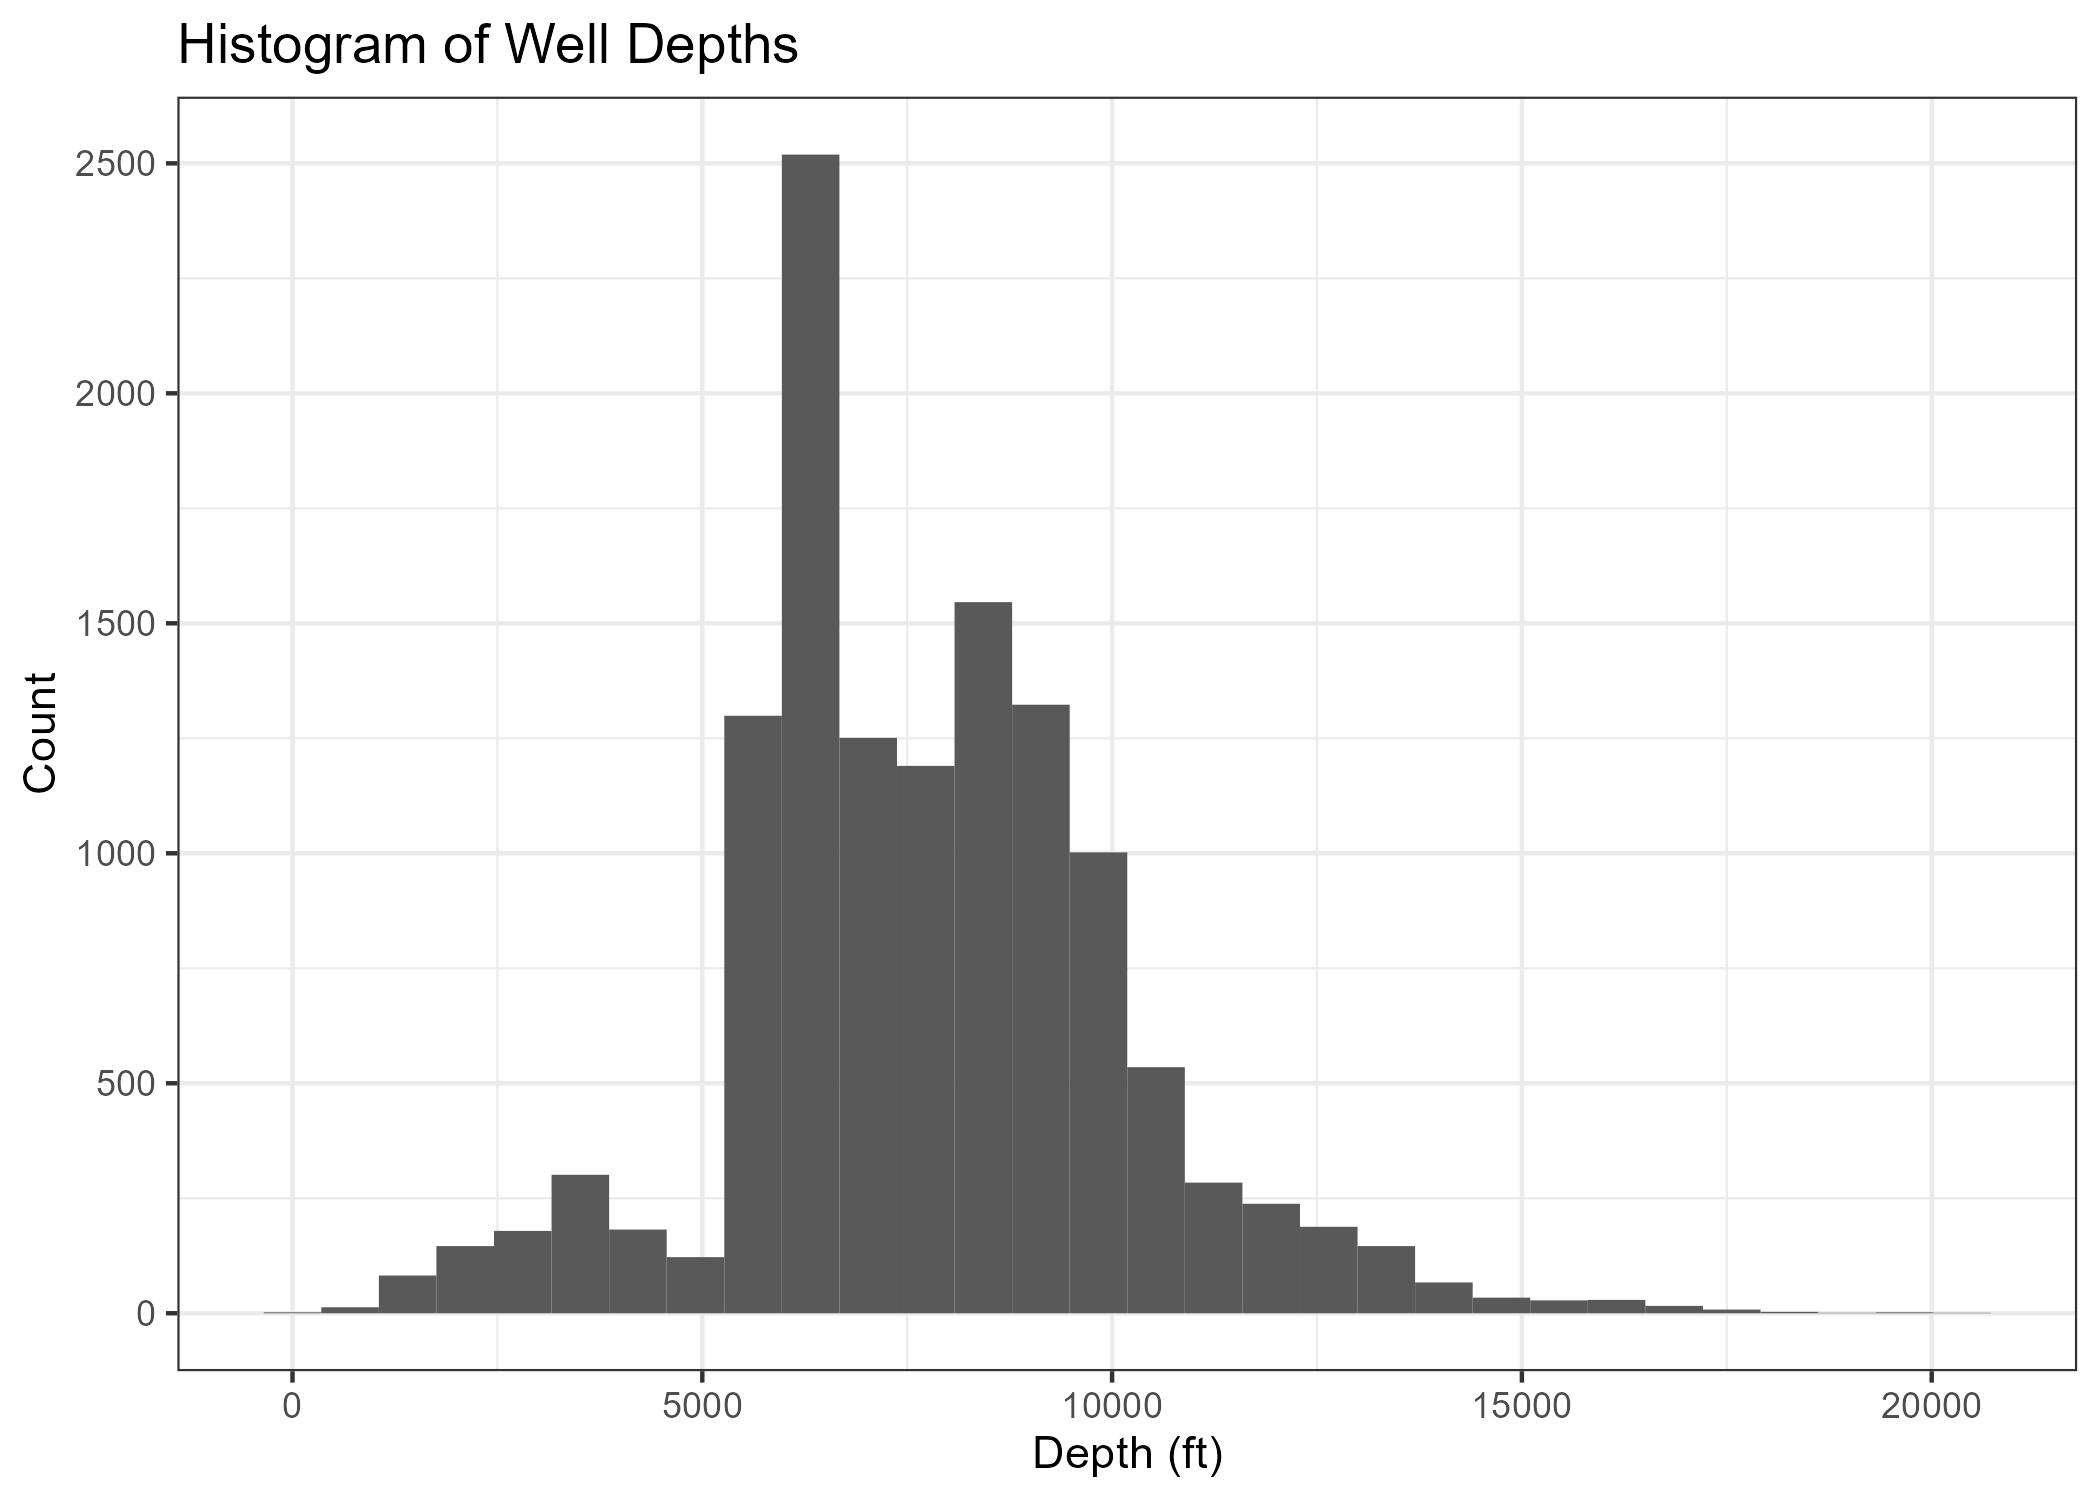
\includegraphics[scale=0.12]{Figures/DepthHistogram.jpg}\\
    \hyperlink{costcalc}{\beamerskipbutton{Back}}
\end{frame}

\begin{frame}{Zoomed Plot: $\$37,500$ per well costs}
\label{Liability1Zoom}
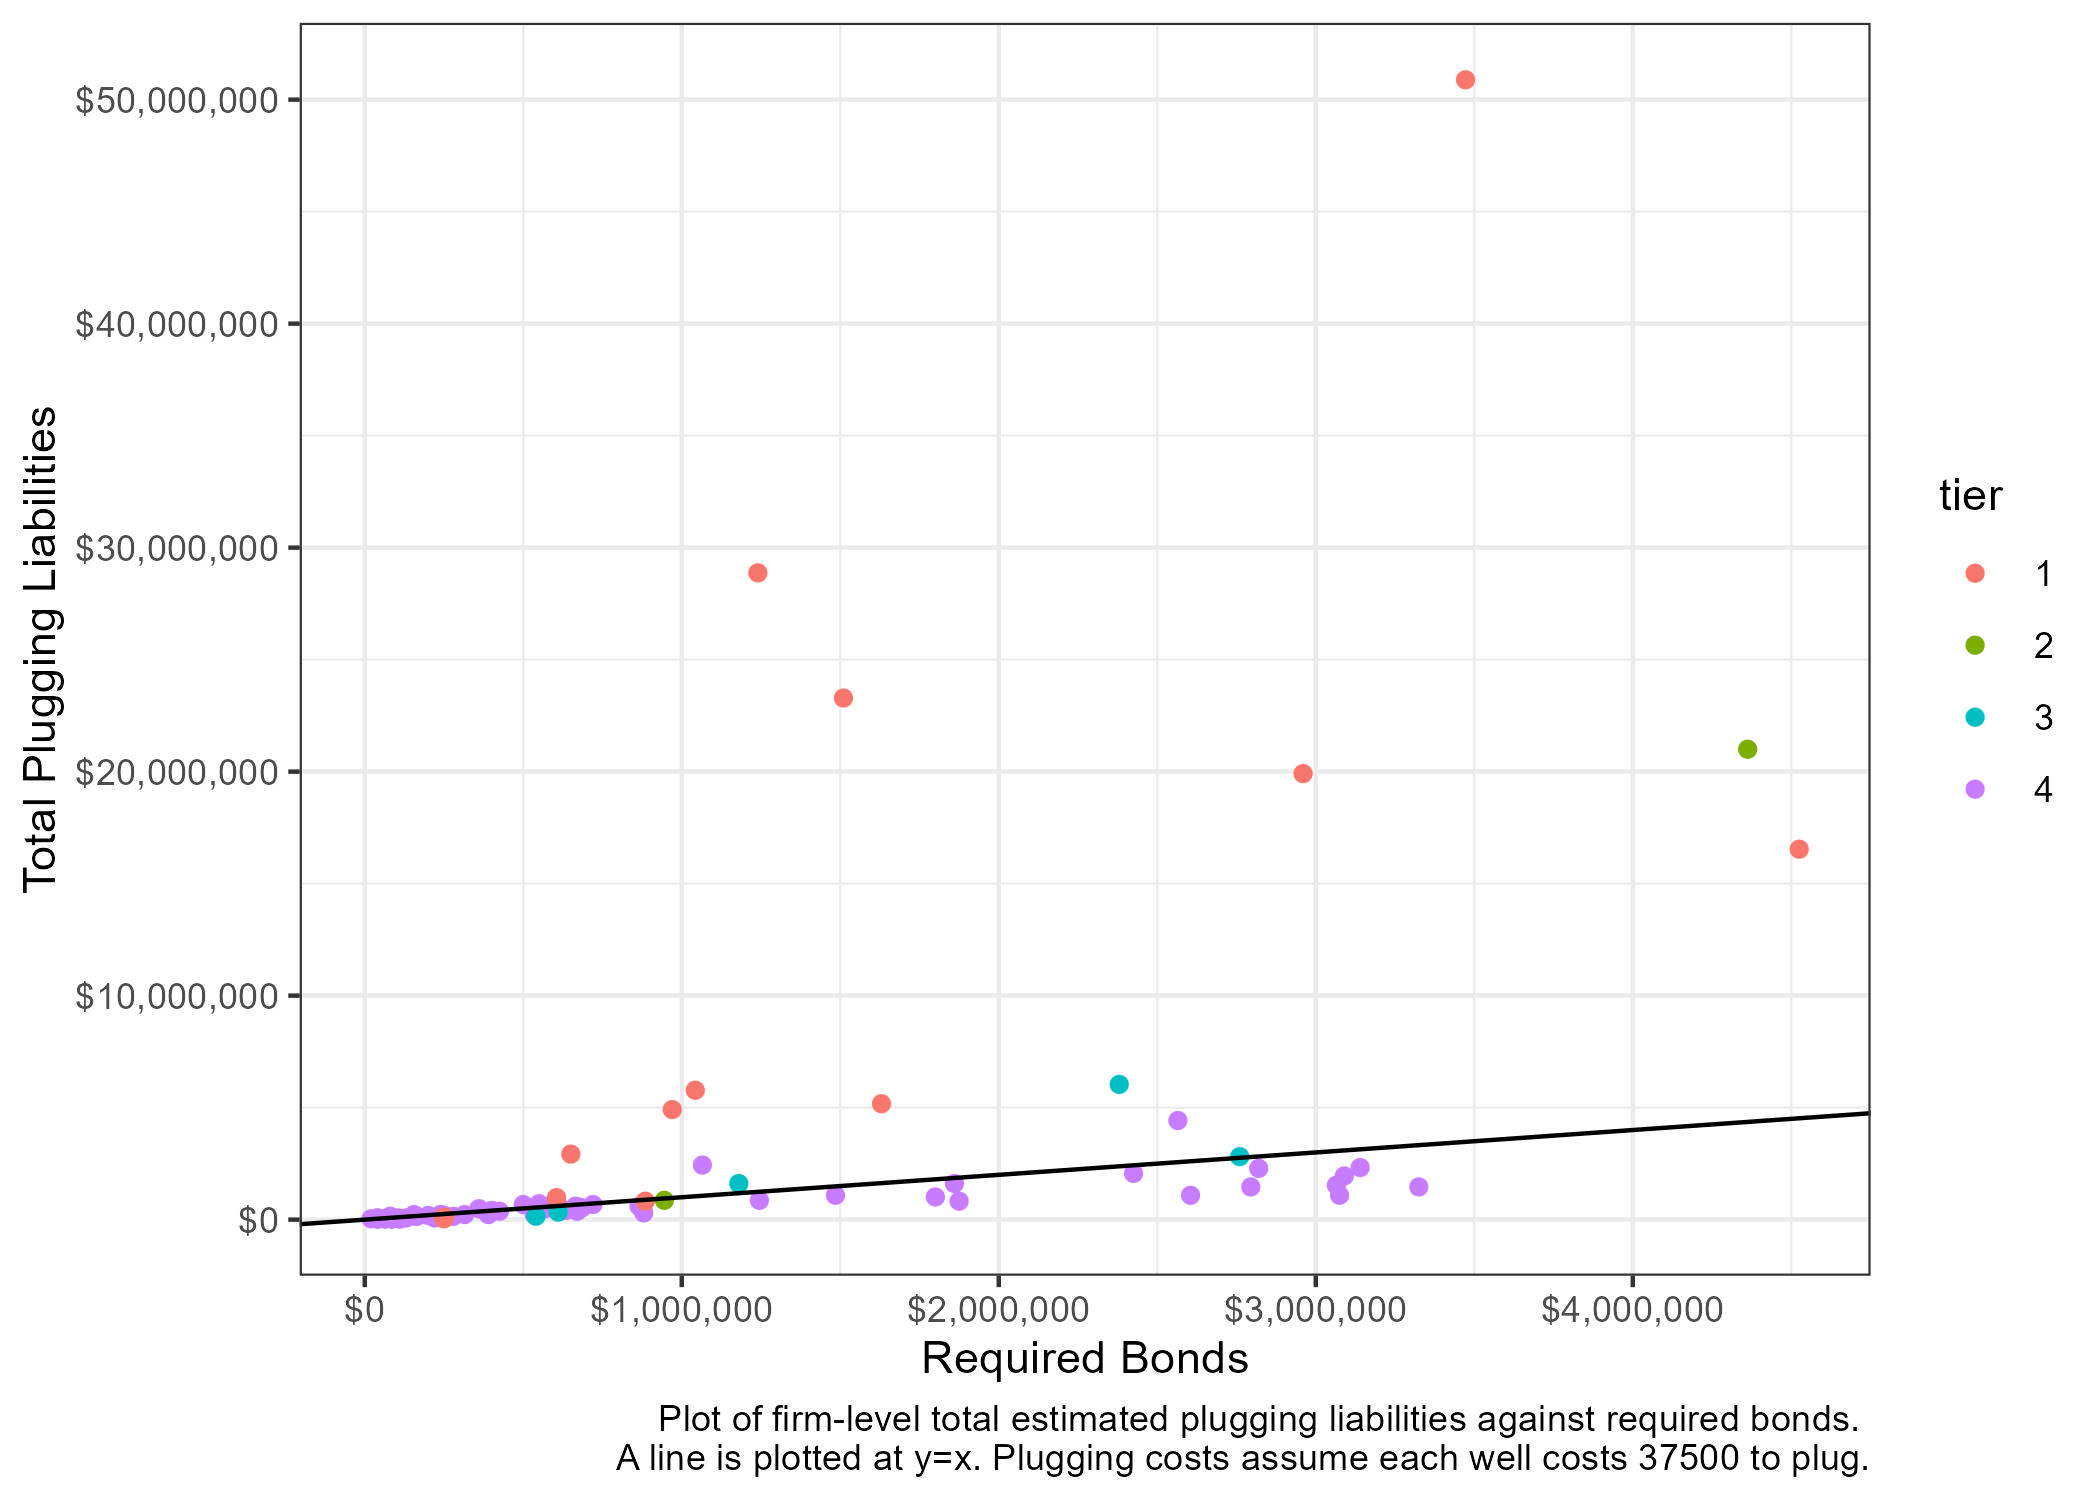
\includegraphics[width=0.8\textwidth]{Figures/BondsLiabilities1_zoomed.jpg}\\
\hyperlink{Fig1}{\beamerskipbutton{Back}}
\end{frame}


\begin{frame}{Zoomed Plot: $\$75,000$ per well costs}
\label{Liability2Zoom}
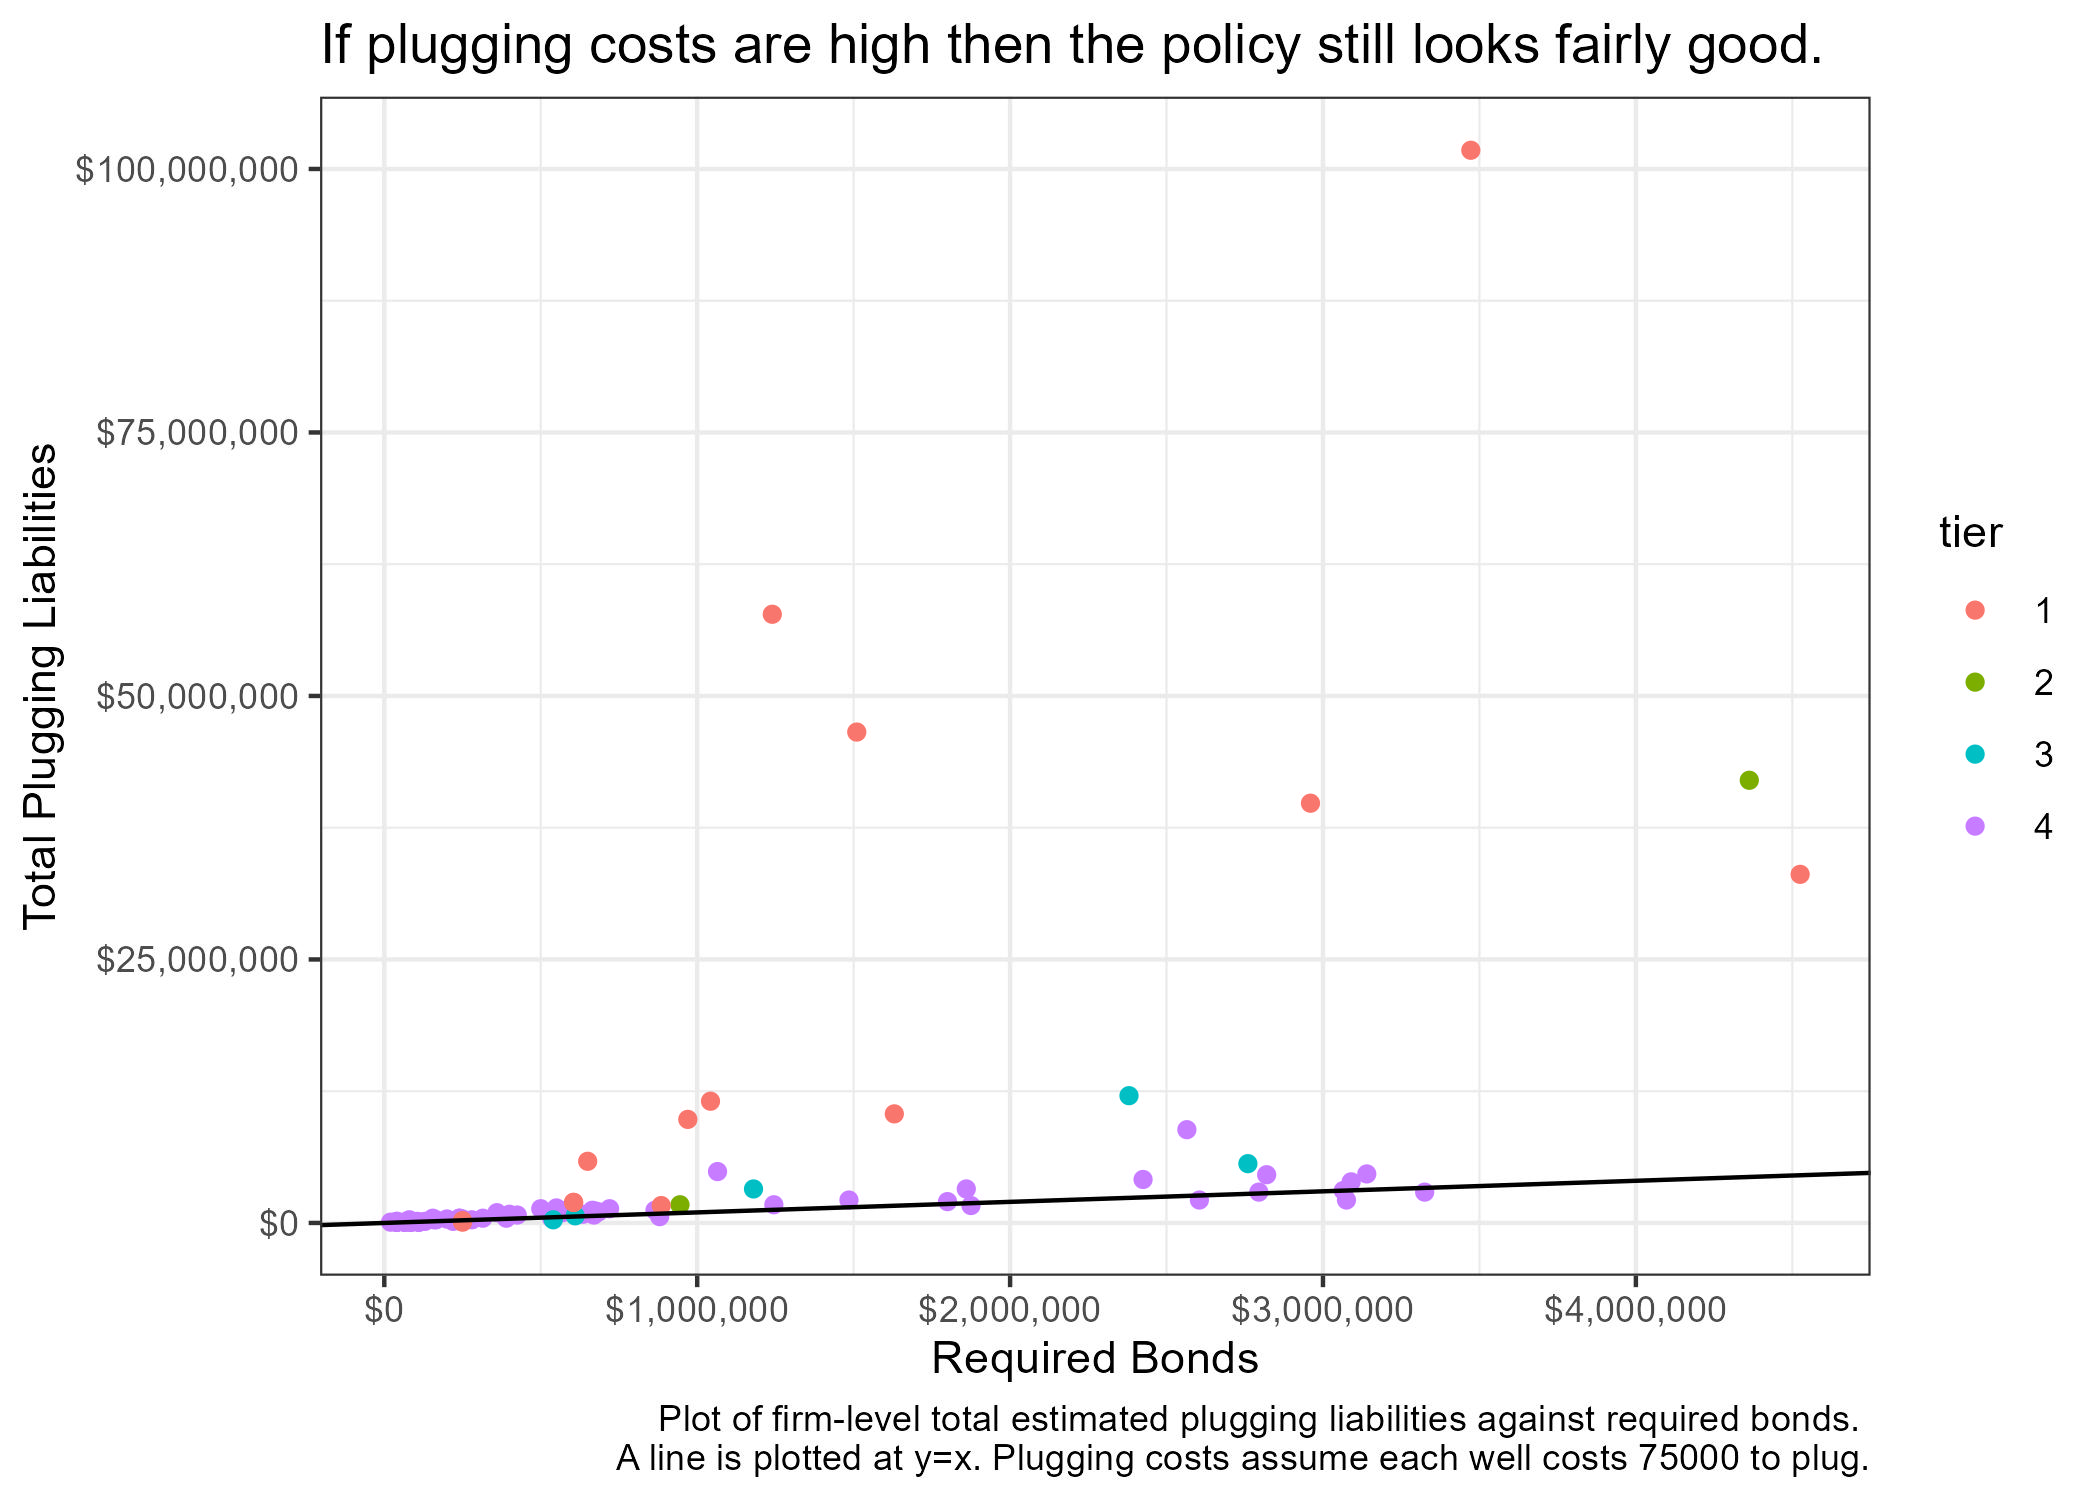
\includegraphics[width=0.8\textwidth]{Figures/BondsLiabilities2_zoomed.jpg}\\
\hyperlink{Fig2}{\beamerskipbutton{Back}}
\end{frame}

\begin{frame}{Marginal/Inactive Plugging Liabilities For Non-Tiered Firms}
\label{Tier4Liability2}
\vspace{-0.3cm}
    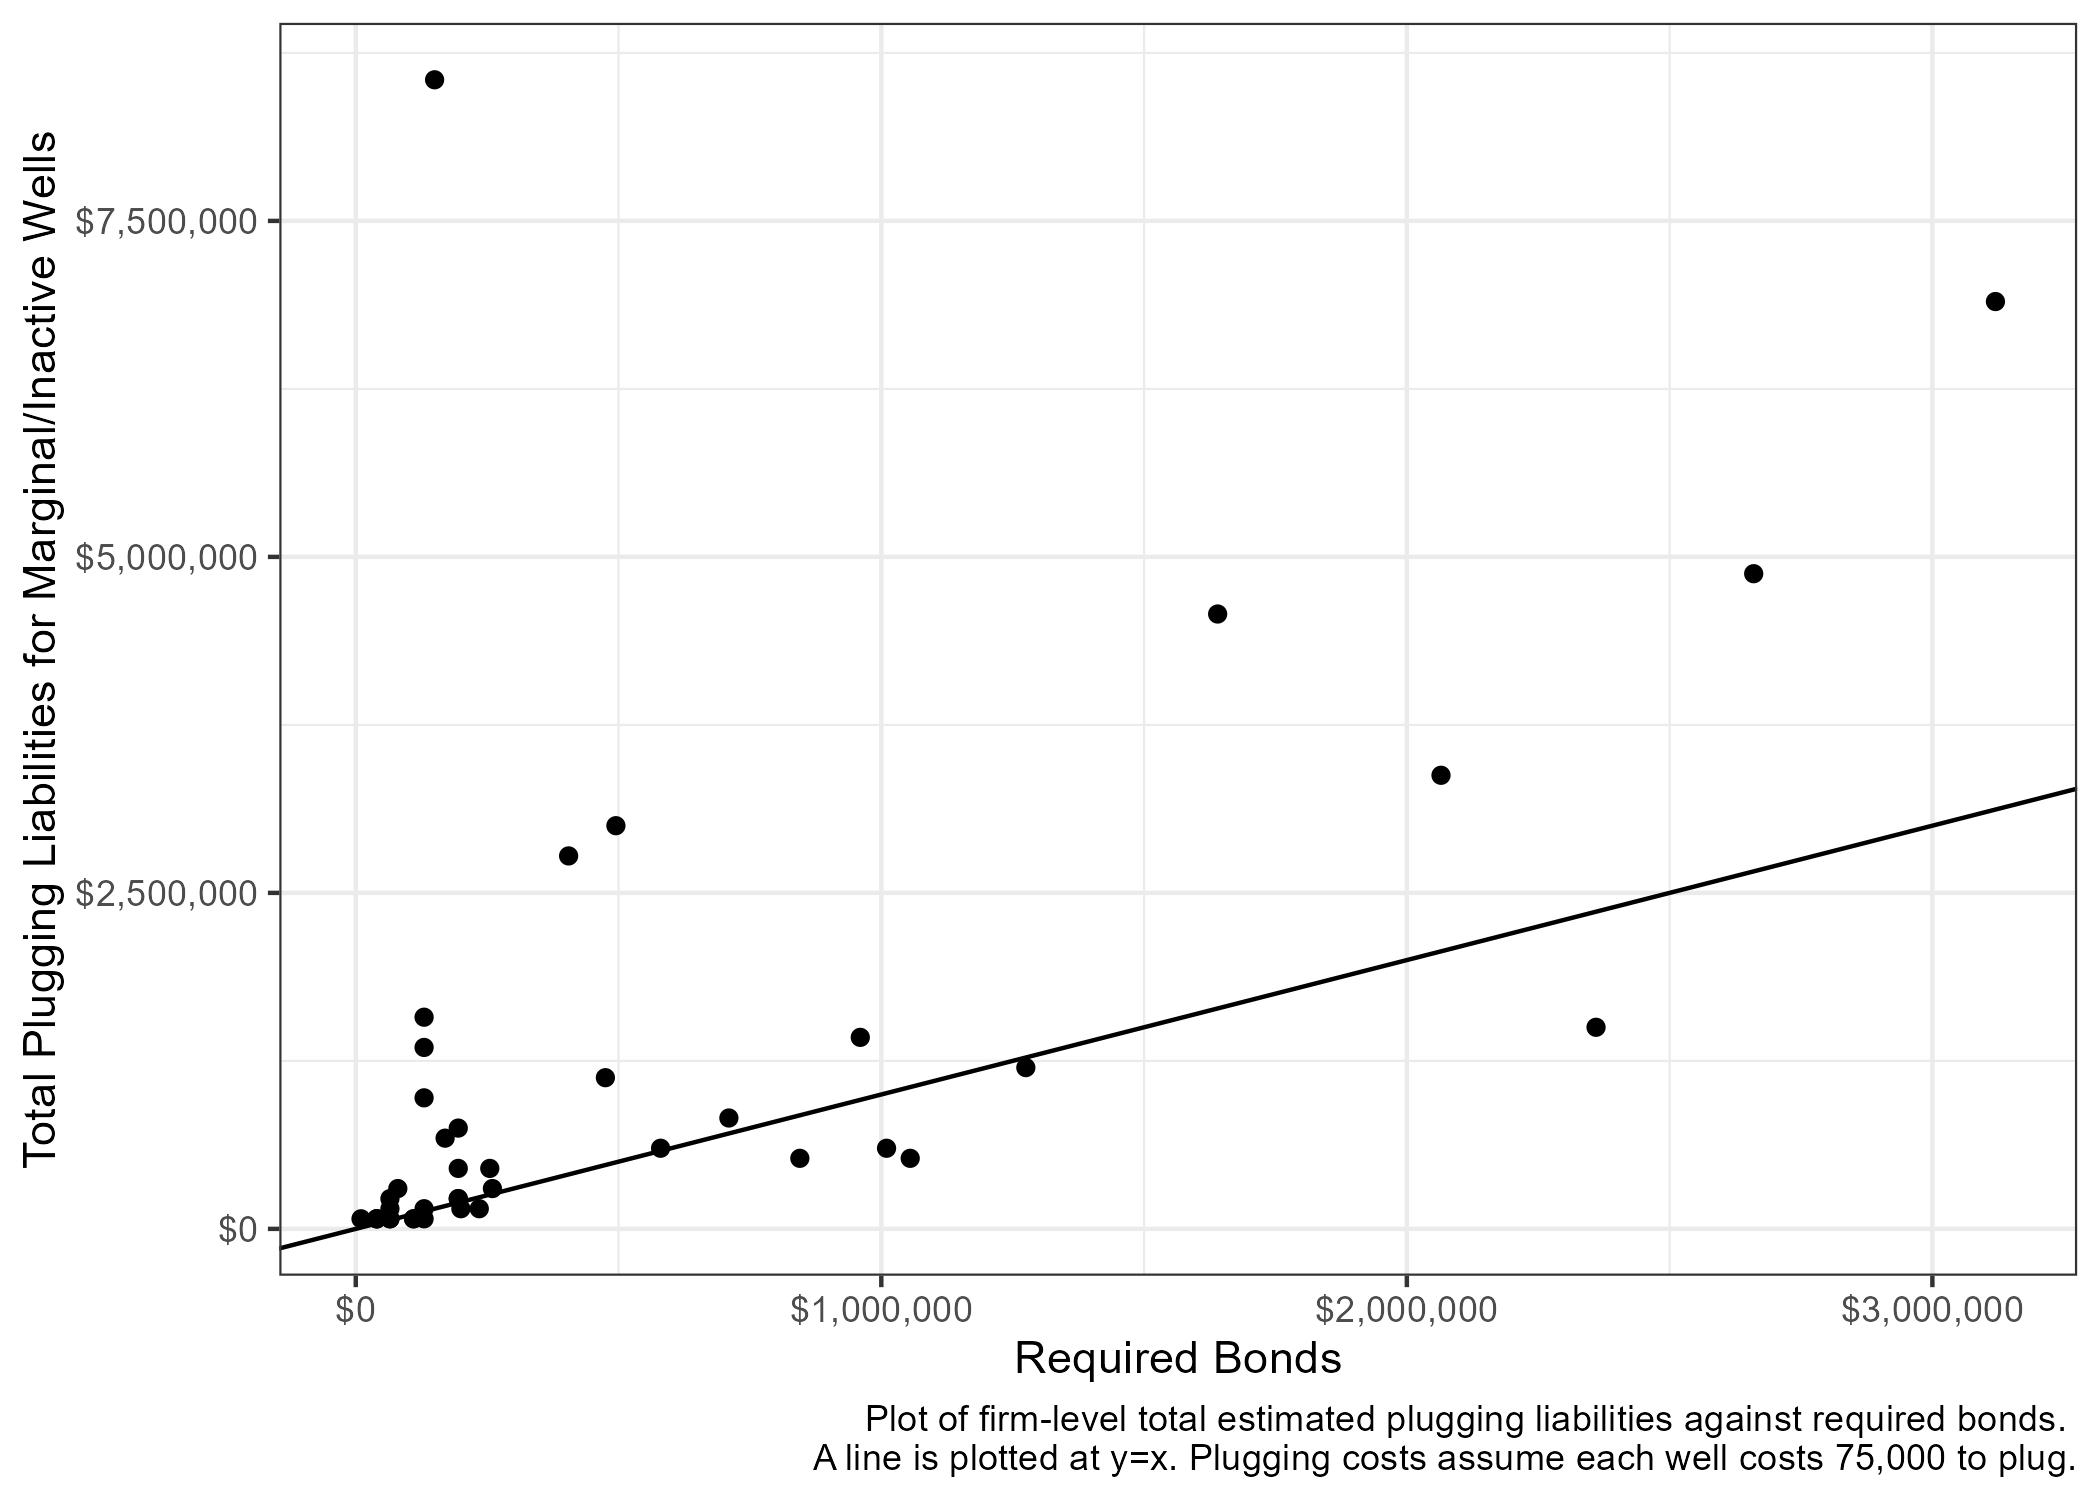
\includegraphics[width=0.8\textwidth]{Figures/InactiveMarginalLiabilities2_Tier4SmallFirms.jpg}

    \hyperlink{Fig2Marginal}{\beamerskipbutton{Back}}
\end{frame}

\begin{frame}{$\$6$ per foot to plug}
\label{MarginalInactiveLiability3}
    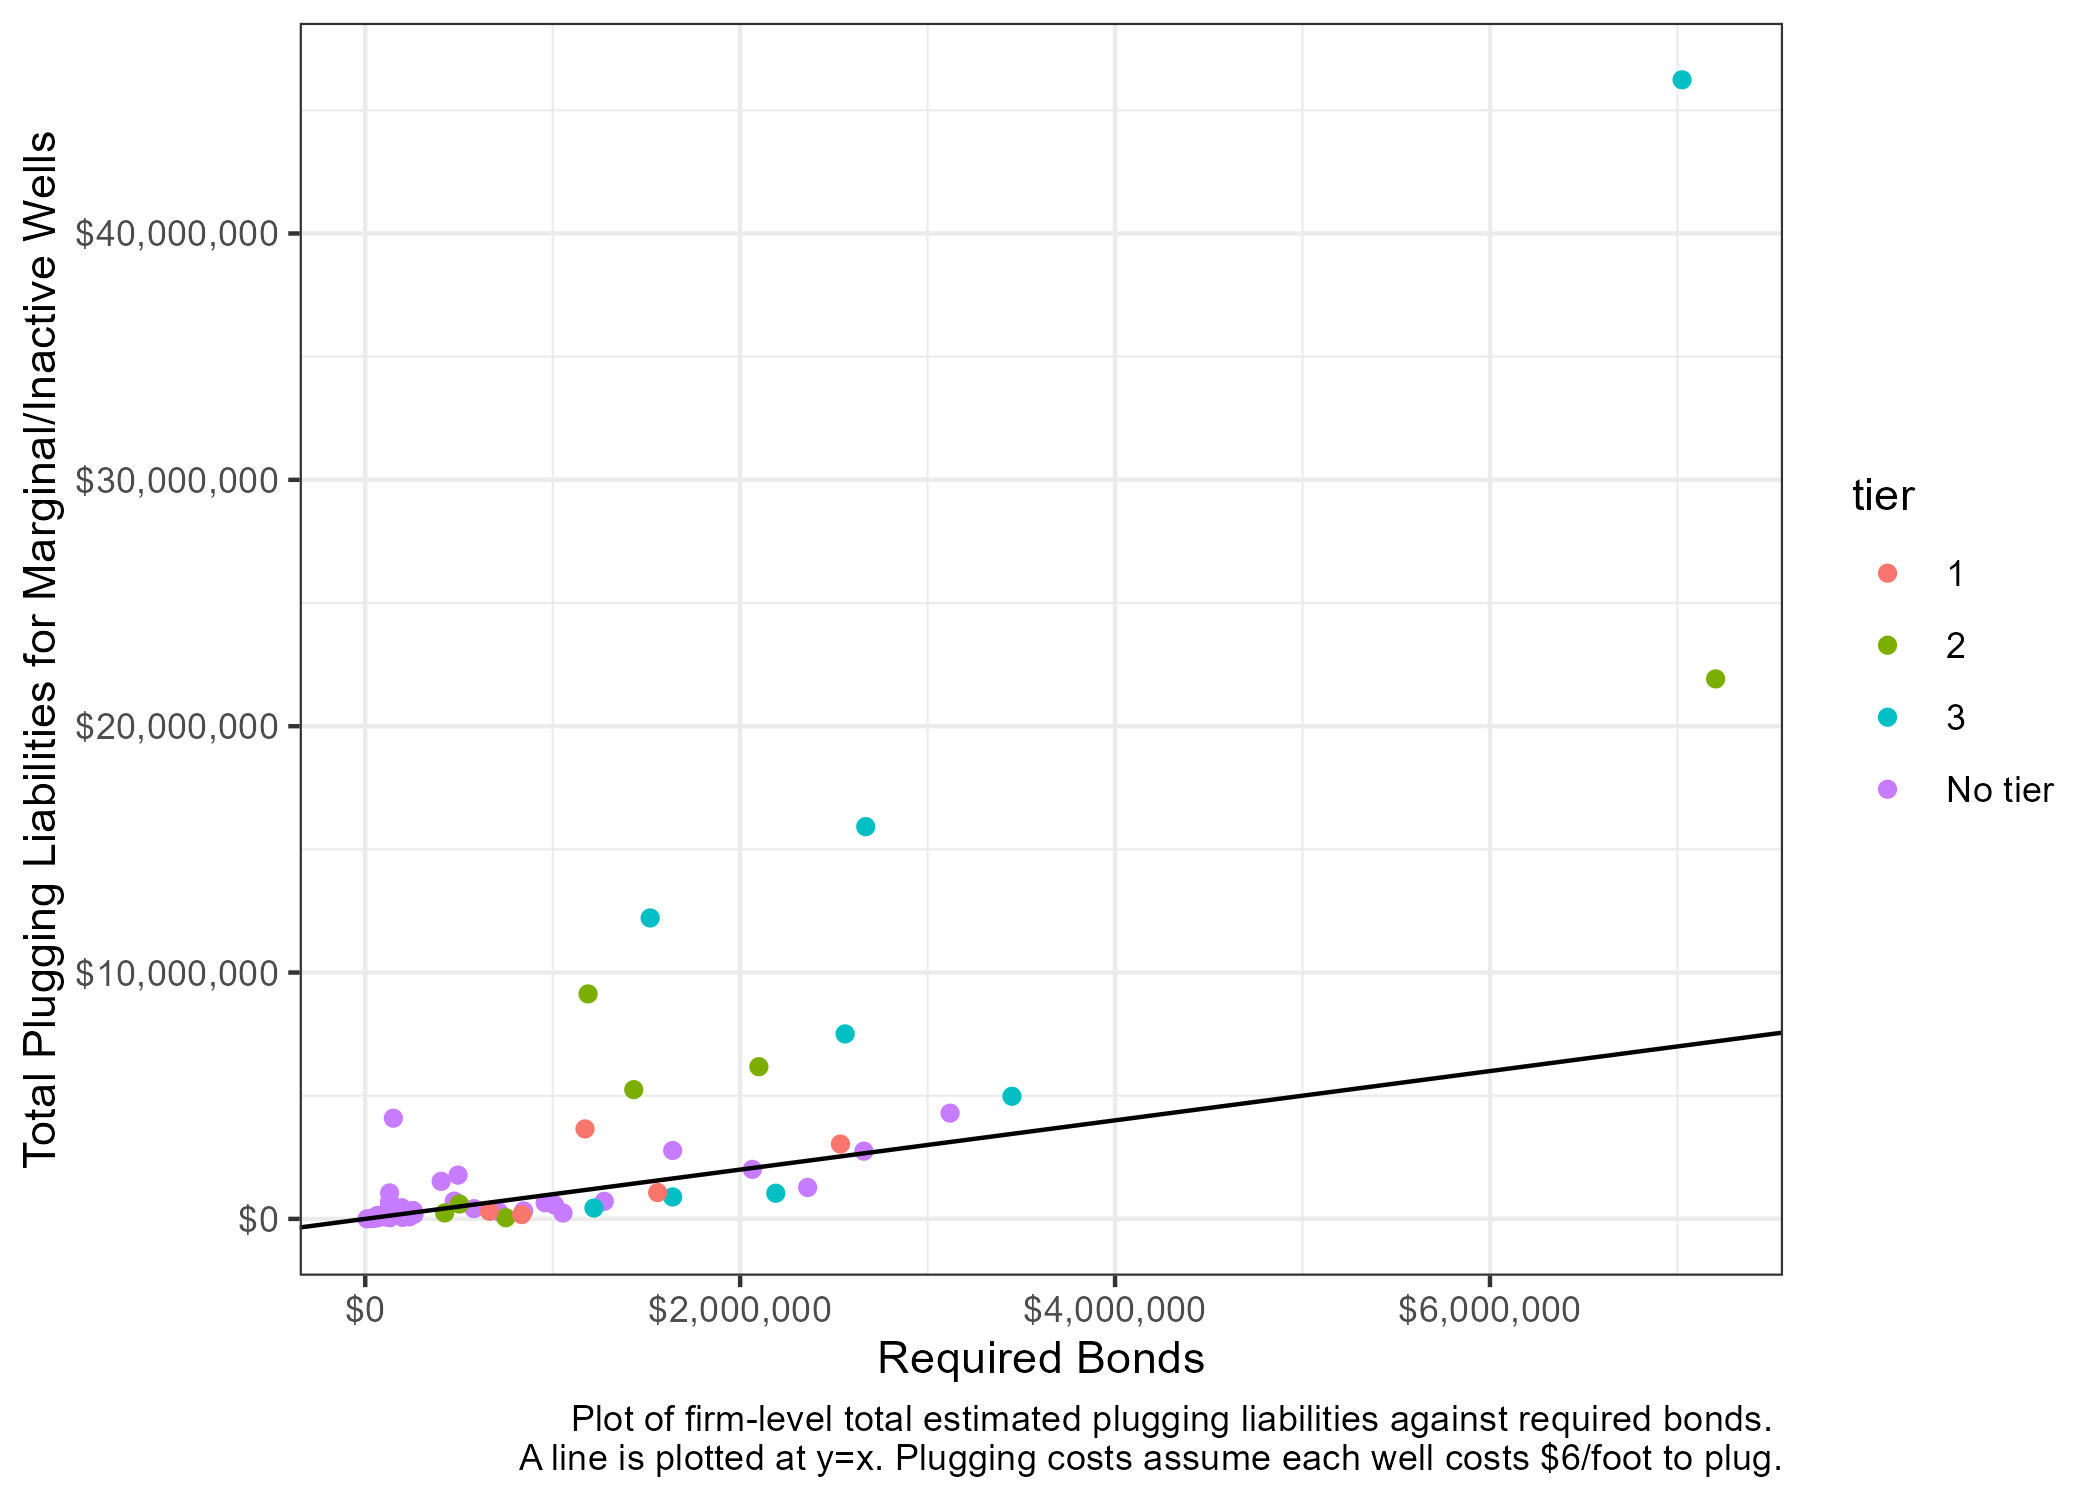
\includegraphics[width=0.8\textwidth]{Figures/InactiveMarginalLiabilities3.jpg}
\end{frame}

\begin{frame}{$\$12$ per foot to plug}
    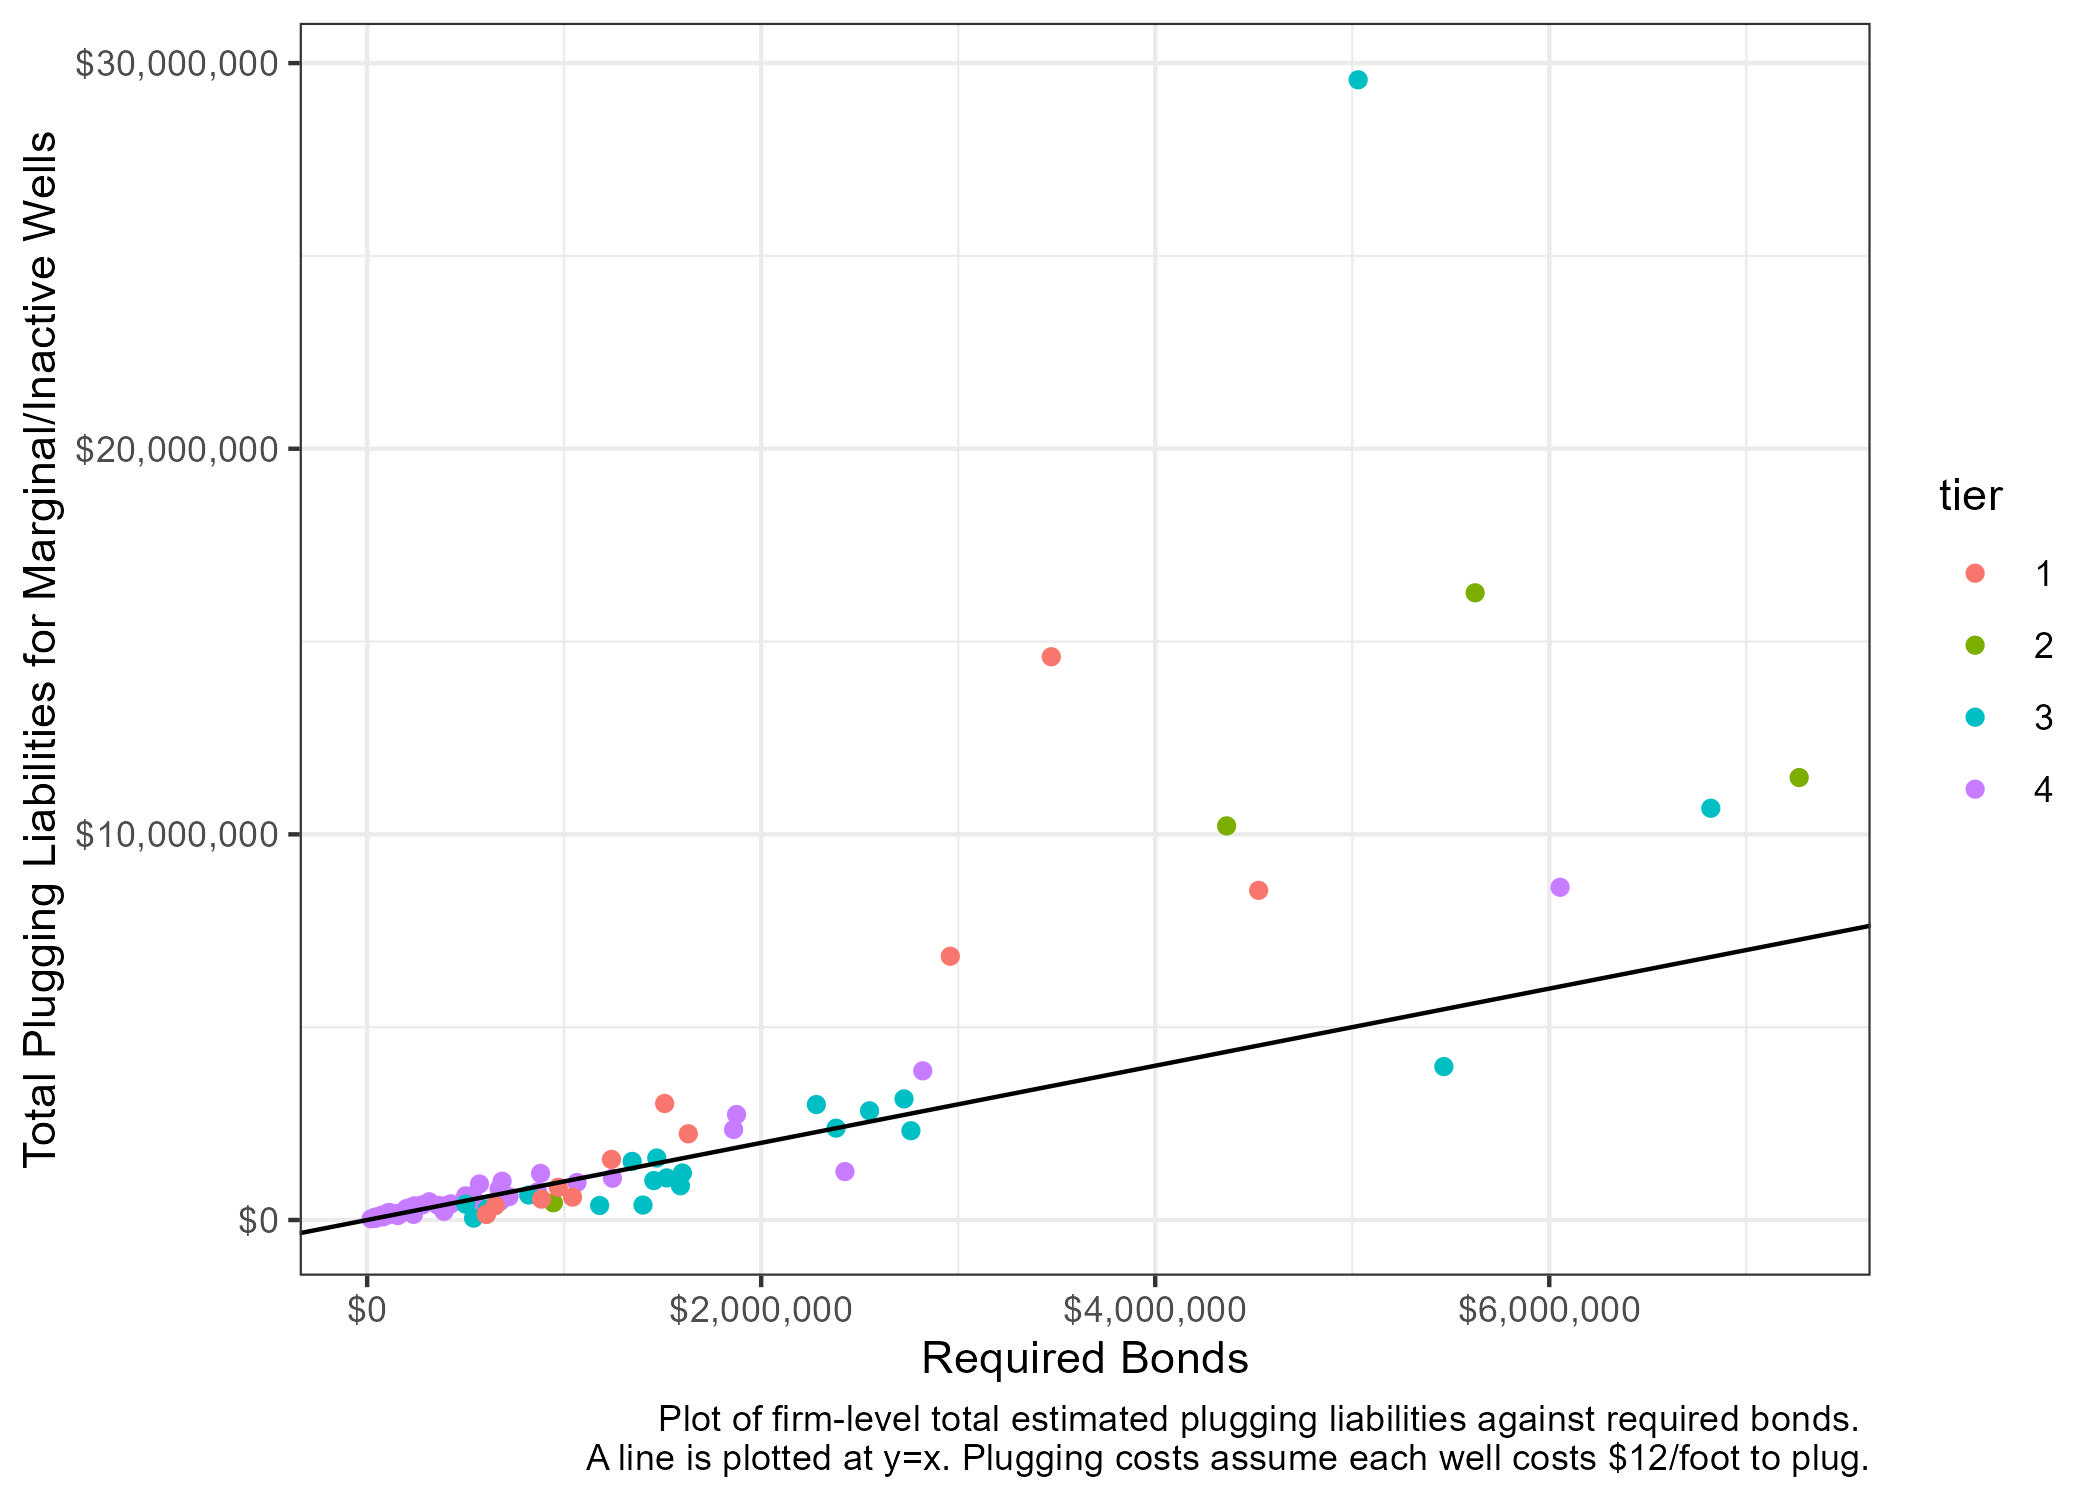
\includegraphics[width=0.8\textwidth]{Figures/InactiveMarginalLiabilities4.jpg}\\
    \hyperlink{Thanks}{\beamerskipbutton{Back}}
\end{frame}

\begin{frame}{UPA Tier Suggestions}
\label{UPA}
\begin{columns}
    \column{0.5\linewidth}{The Utah Petroleum Association (UPA) submitted a comment in support of moving each of the inactive/marginal well tier thresholds up by $5\%$ each.
    \begin{itemize}
        \item Tier 1: $<20\%$ inactive/marginal wells and $>1,000$ BOE/day
        \item Tier 2: $<25\%$ inactive/marginal wells and $>500$ BOE/day
        \item Tier 3: $<30\%$ inactive/marginal wells and $>200$ BOE/day \textbf{OR} $>1000$ BOE/day
    \end{itemize}}
    \column{0.6\linewidth}{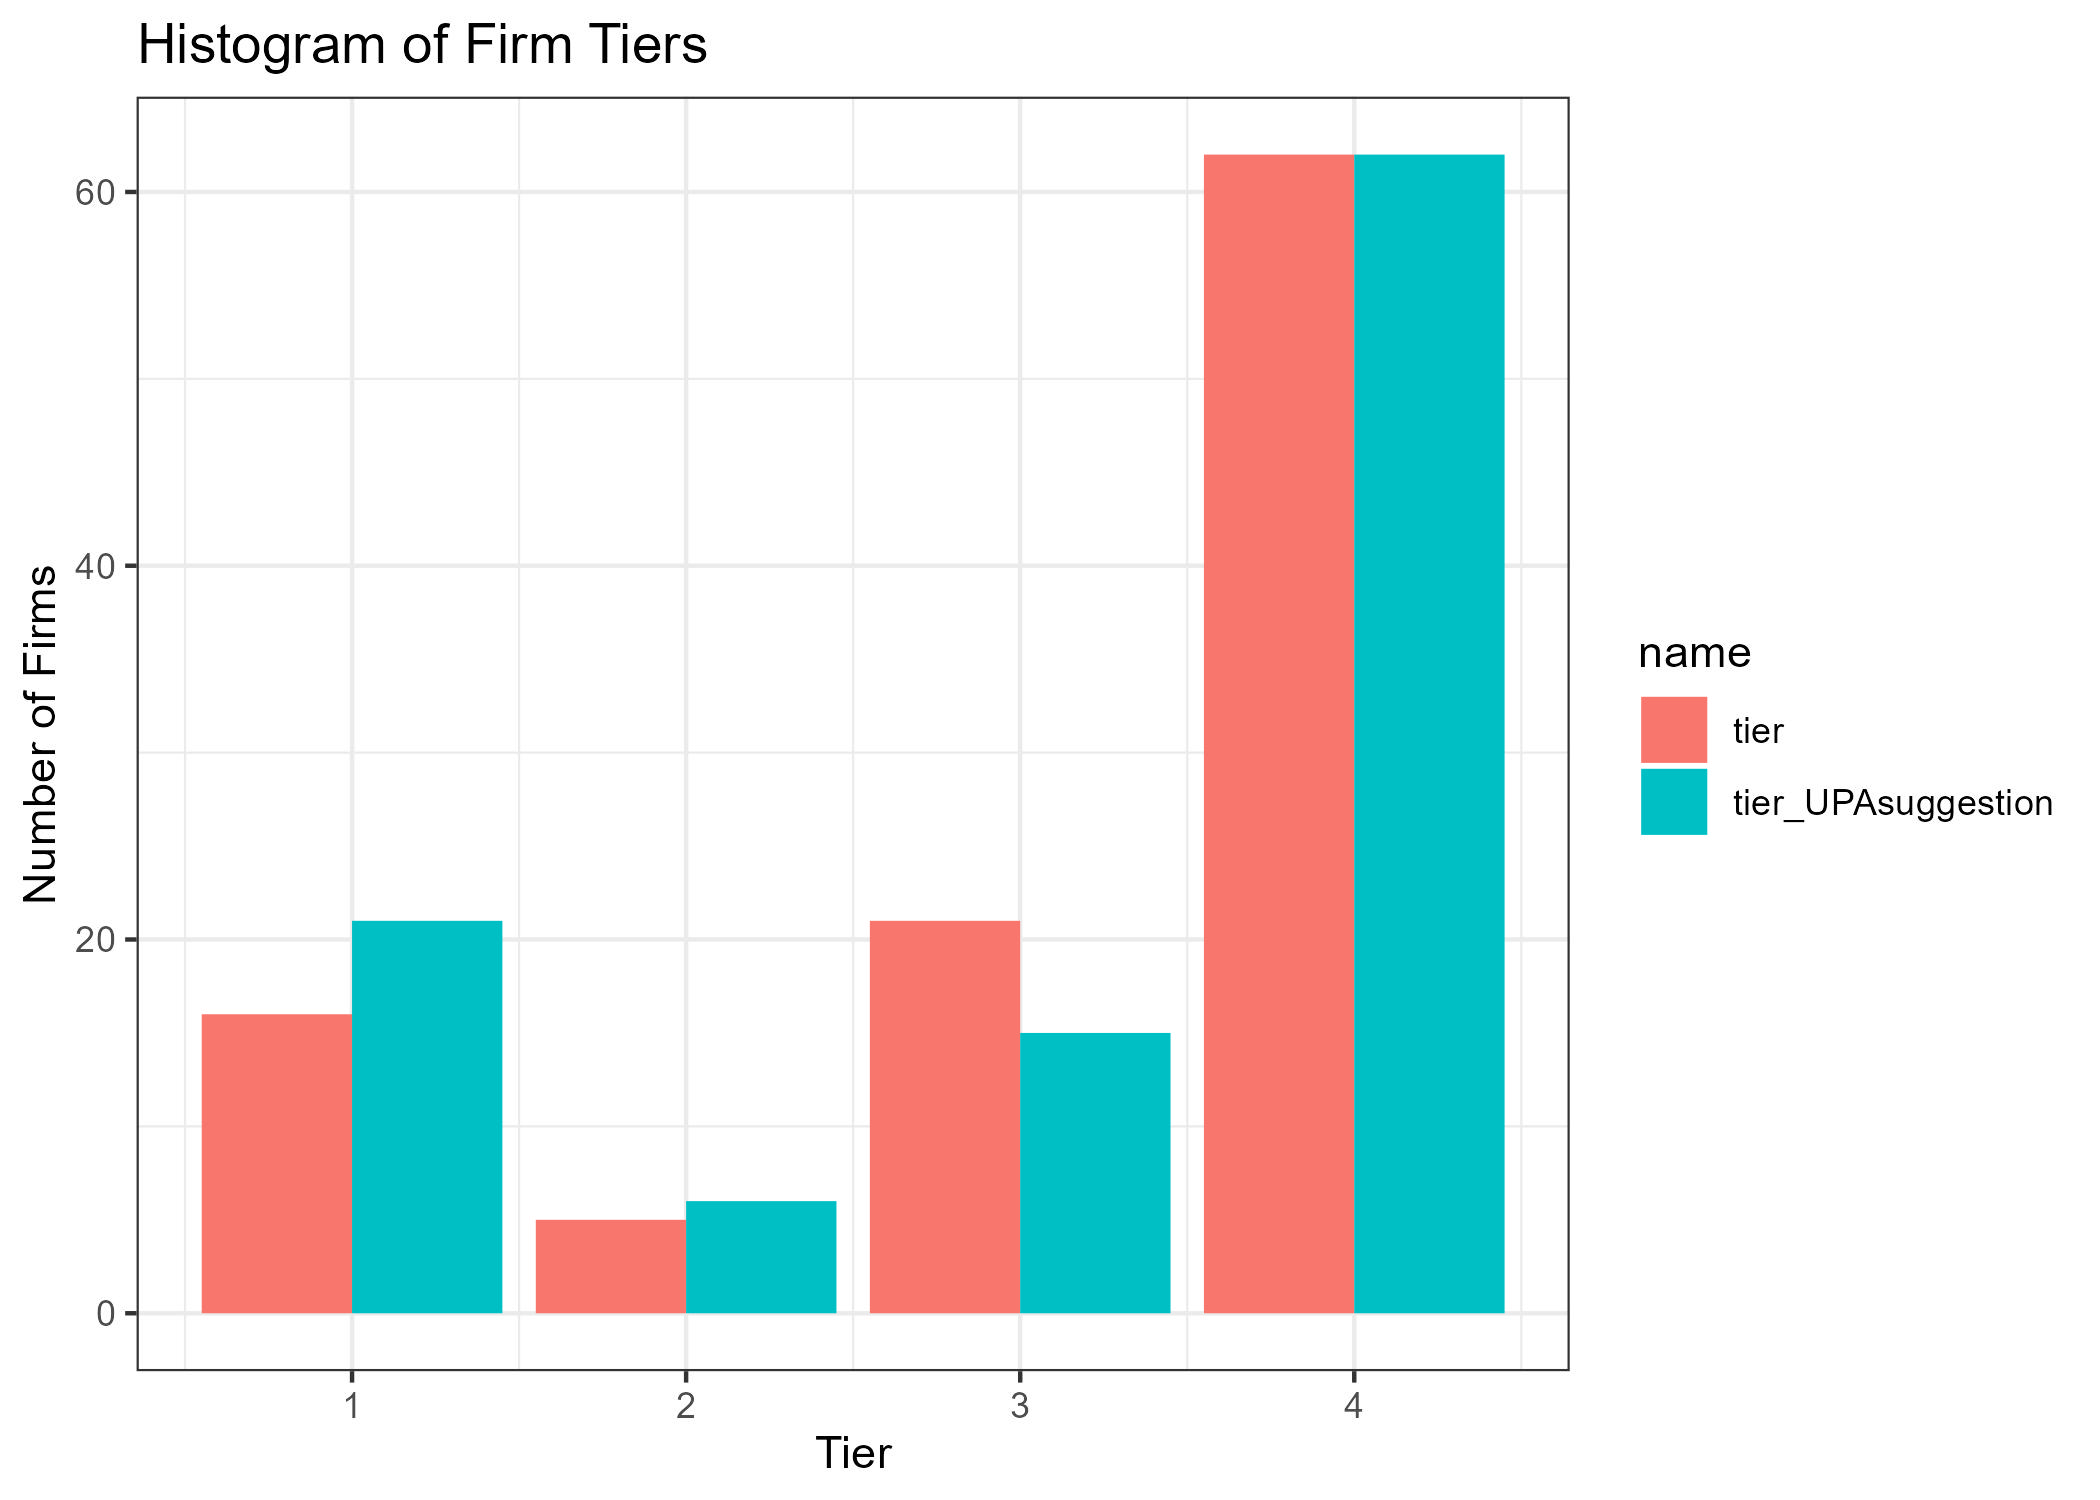
\includegraphics[width=\textwidth]{Figures/Histogram_Tiers_UPAsuggestion.jpg}}
\end{columns}
    
\end{frame}

\begin{frame}{UPA Tier Suggestions}
\label{UPA}
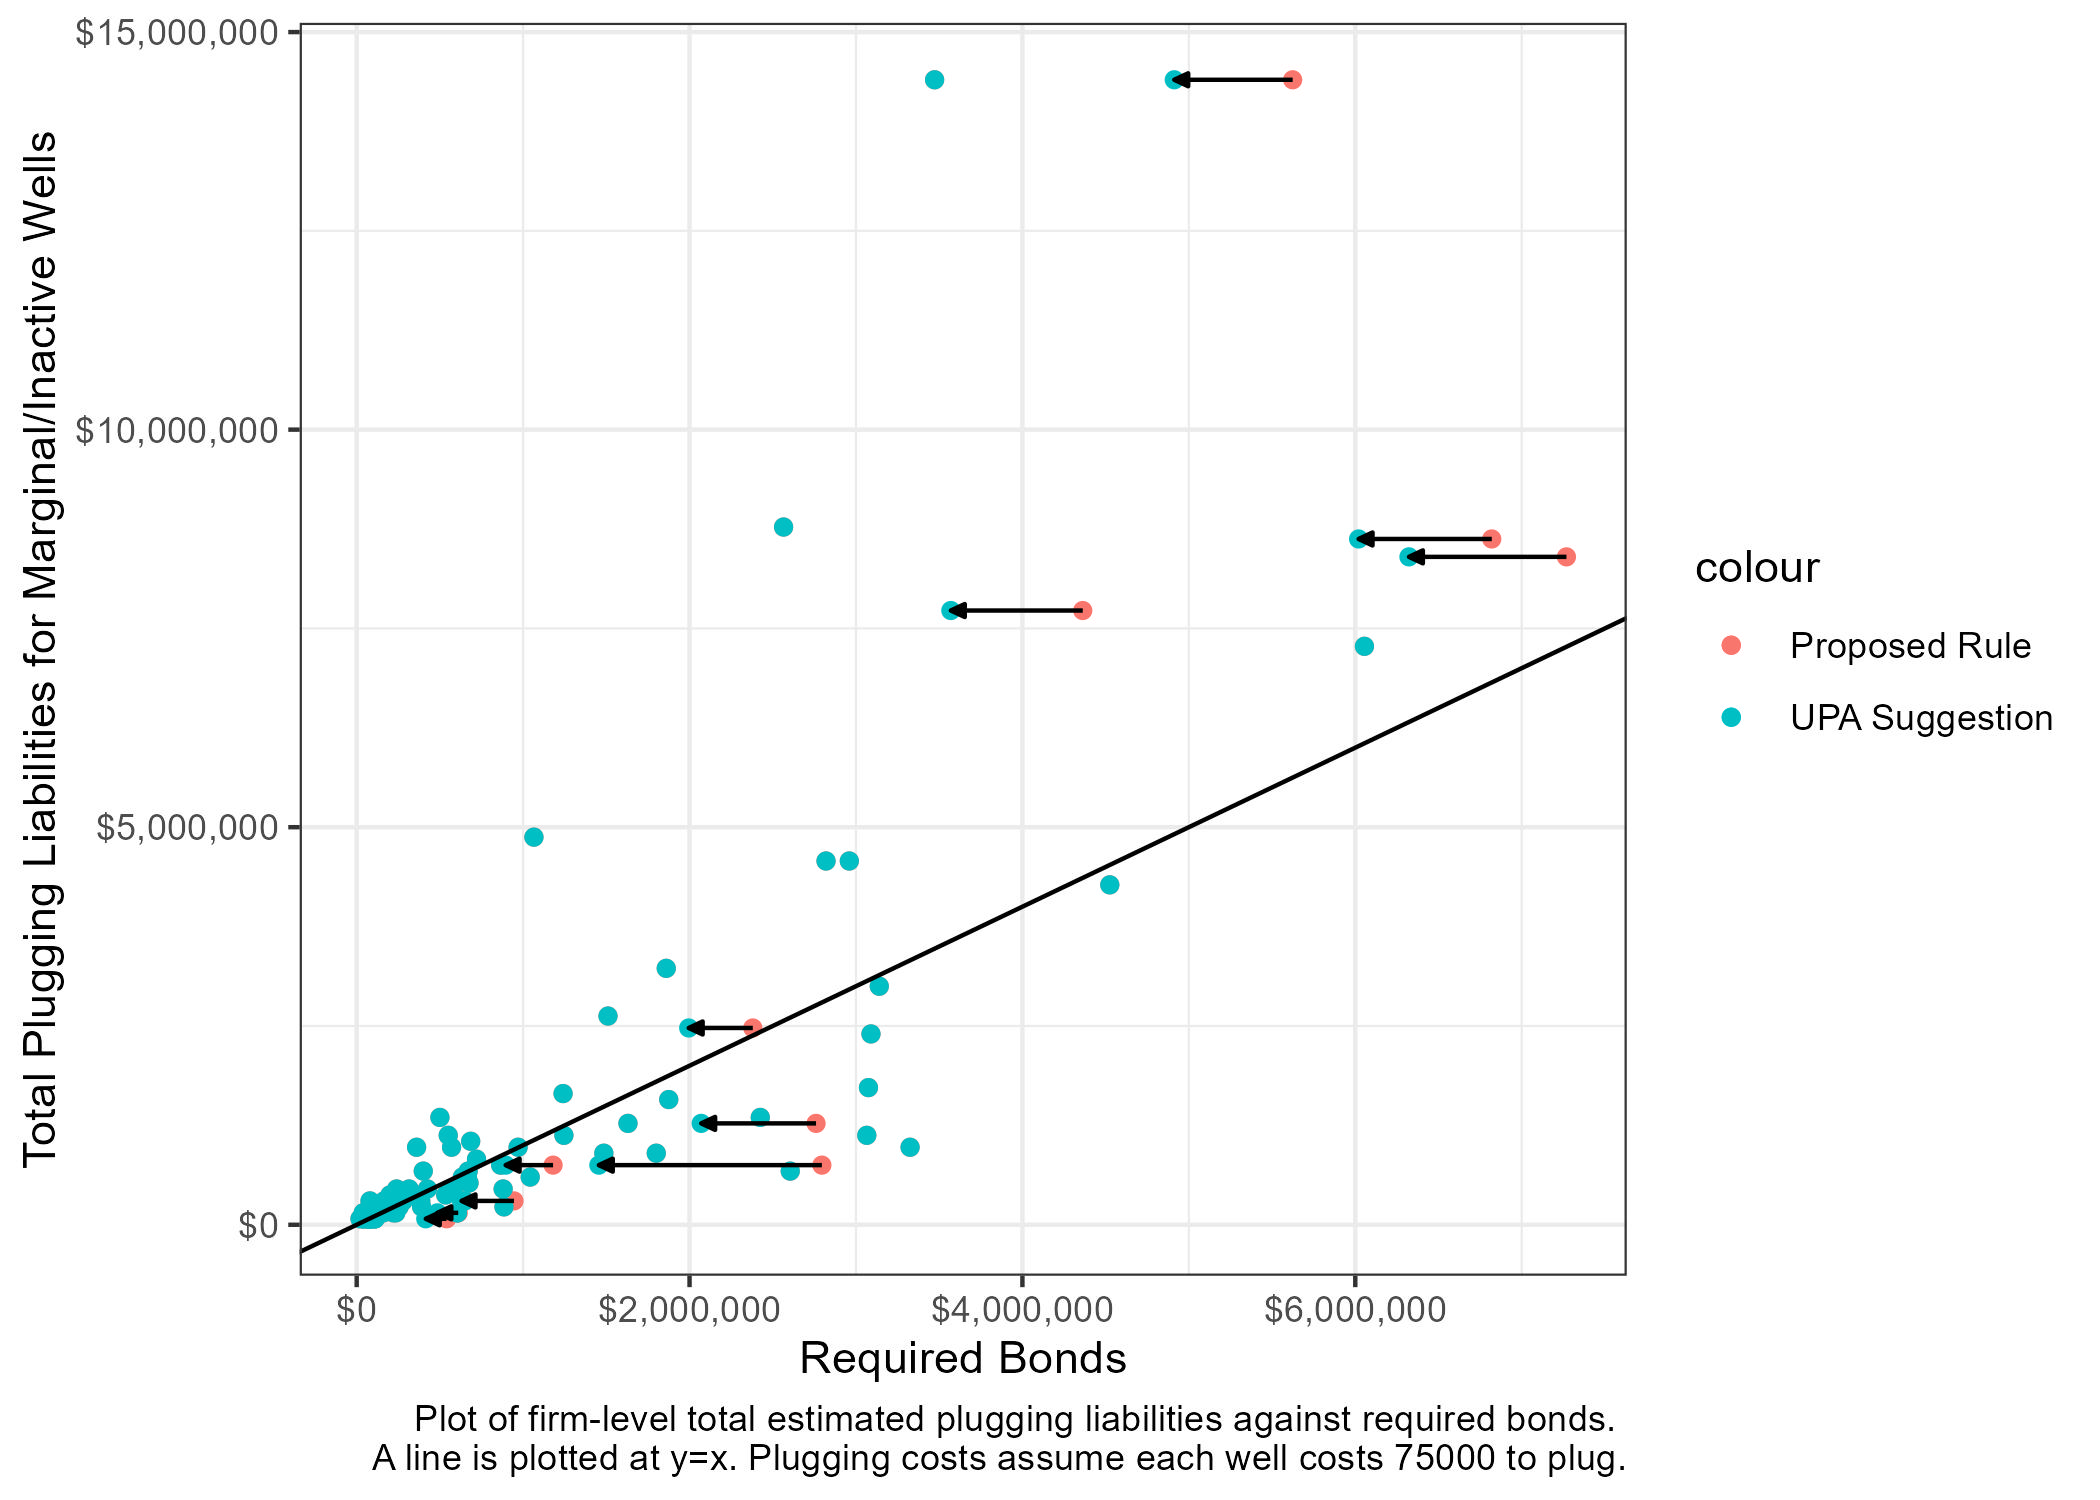
\includegraphics[width=0.8\textwidth]{Figures/UPA_Suggestion_Bond_Changes.jpg}\\
\hyperlink{Thanks}{\beamerskipbutton{Back}}
\end{frame}

\end{document}